\documentclass{article}
\usepackage[utf8]{inputenc}
\usepackage[margin=1.5cm]{geometry}
\usepackage{amsmath}
\usepackage{amssymb}
\usepackage{xcolor}
\definecolor{oxblue}{RGB}{0, 0, 51}
\usepackage{graphicx}
\usepackage{caption}
\usepackage{float}
\usepackage[sc]{titlesec}
\usepackage{tasks}
\usepackage{enumitem}
\newcommand{\dd}[1]{\mathrm{d}#1}
\renewcommand{\arraystretch}{1.5}

\titleformat{\section}{\centering\Large\scshape}{\thesection \ }{0.5em}{}
\titleformat{\subsection}{\centering\large\scshape}{}{0em}{}


\begin{document}

\title{\Huge\textsc{JLI Maths Workbook Solutions}}
\author{J.J. Winterburn}
\date{}

\maketitle
\thispagestyle{empty}

\begin{center}
  \textsc{\large{Comments and corrections to jjw79@cam.ac.uk}}
\end{center}

\clearpage

\pagenumbering{arabic}

\section{Review of Algebra}
\noindent

1.

$$
  C(q) = 4 + 2q + \frac{1}{2}q^2
$$

$$
  C(4) = 20
$$

$$
  C(1) = \frac{13}{2}
$$

$$
  C(0) = 4
$$

2.

$$
  (-2)^3 \cdot (-10+7) = -8 \cdot -3 = 24
$$

3.

\begin{center}
  \begin{tabular}{ c c }
    a) $3x(x+y-5)$ & b) $2\left( z^3+z-6 \right)$
  \end{tabular}
\end{center}

4.

\begin{center}
  \begin{tabular}{ c c c }
    a) $\frac{6a^4b \cdot 4b}{8ab^3c} = \frac{3a^3}{bc}$ & b) $\sqrt{\frac{3x^3y}{27xy}} = \sqrt{\frac{x^2}{9}} = \pm \frac{x}{3}$ & c) $\left( 2x^3 \right)^3 \cdot \left( xz^2 \right)^4 = 8x^9 \cdot x^4z^8 = 8x^{13}z^8$
  \end{tabular}
\end{center}


5.
\begin{center}
  \begin{tabular}{ c c }
    a) $\frac{2y}{3x} + \frac{4y}{5x} = \frac{22y}{15x}$ & b) $\frac{x+1}{4} - \frac{2x-1}{3} = \frac{7-5x}{12}$
  \end{tabular}
\end{center}

6.

\begin{center}
  \begin{tabular}{ c }
    a) $x^2-7x+12 = (x-3)(x-4)$ \\ b) $16y^2-25 = (4y+5)(4y-5)$ \\ c) $3z^2-10z-8 = (3z+2)(z-4)$
  \end{tabular}
\end{center}

7.

\begin{center}
  \begin{tabular}{ c c c }
    a) $4^{\frac{3}{2}} = 8$ & b) $\log_{10}100 = 2$ & c) $\log_{5}125 = 3$
  \end{tabular}
\end{center}

8.

\begin{center}
  \begin{tabular}{ c c }
    a) $2\log_a(3x)+\log_ax^2 = \log_a9x^4$ & b) $\log_ay-3\log_az = \log_a\left( \frac{y}{z^3} \right)$
  \end{tabular}
\end{center}

9.

\begin{center}
  \begin{tabular}{ c }
    a) $5(2x-9) = 2(5-3x) \implies 16x = 55 \implies x = \frac{55}{16}$ \\
    b) $1+\frac{6}{y-8} = -1 \implies y-8 + 6 = 8 - y \implies y = 5$ \\
    c) $z^{\frac{2}{5}}=7 \implies z=7^{\frac{5}{2}}$ \\
    d) $3^{2t-1}=4 \implies (2t-1)\ln{3}=\ln{4} \implies 2t-1 = \frac{\ln{4}}{\ln{3}} \implies t = \frac{1}{2}\left( 1+\frac{\ln{4}}{\ln{3}} \right)$
  \end{tabular}
\end{center}

10.

\begin{center}
  \begin{tabular}{ c }
    a) $ax-7a=1 \implies x=\frac{1+7a}{a}$ \\
    b) $5x-a = \frac{x}{a} \implies x\left( 5-\frac{1}{a}=a \right) \implies x = \frac{a^2}{5a-1}$ \\
    c) $\log_a{2x+5} = 2 \implies 2x+5 = a^2 \implies x = \frac{a^2-5}{2}$
  \end{tabular}
\end{center}

11.

$$
  P = \sqrt{\frac{a}{Q^2+b}} \implies P^2 = \frac{a}{Q^2+b} \implies Q^2 = \frac{a}{P^2}-b \implies Q=\sqrt{\frac{a}{P^2}-b}
$$

12.

\begin{center}
  \begin{tabular}{ c }
    a) $2x^2+5x-7=0 \implies (2x+7)(x-1)=0 \implies x=-\frac{7}{2} \text{ or } x=1$ \\
    b) $y^2+3y-\frac{1}{2}=0 \implies \left( y+\frac{3}{2} \right)^2=\frac{11}{4} \implies y=\frac{-3\pm\sqrt{11}}{2}$
  \end{tabular}
\end{center}

13.\\
\indent
\quad a)

$$
  \begin{matrix}
    2x-y=4 \\
    5x-4y=13
  \end{matrix}
  \implies
  \begin{matrix}
    8x-4y=16 \\
    5x-4y=13
  \end{matrix}
  \implies 13x=29 \implies x=\frac{29}{13},\: y=\frac{6}{13}
$$

\indent
\quad b)

$$
  y = \frac{3x+4}{2} = x^2+1 \implies 2x^2-3x-2=0 \implies (2x+1)(x-2) = 0 \implies x=-\frac{1}{2}\text{ or }x=2
$$

$$
  x=-\frac{1}{2} \iff y=\frac{5}{4}
$$

$$
  x=2 \iff y=5
$$

14.

\begin{center}
  \begin{tabular}{ c }
    a) $2y-7 \leq 3 \implies y \leq 5$ \\
    b) $3-z > 4+2z \implies -1 > 3z \implies -\frac{1}{3}>z$ \\
    c) $3x^2-5x-2<0 \implies (3x+1)(x-2)>0 \implies -\frac{1}{3}<x<2$
  \end{tabular}
\end{center}

\clearpage

\section{Lines and Graphs}

\clearpage

\section{Sequences, Series and Limits; The Economics of Finance}

\subsection{Quick Questions}
\noindent

1.

\begin{center}
  \begin{tabular}{c}
    a) $u_n = 20-5n$ \\
    b) $u_n = n^3$ \\
    c) $u_n = 4u_{n-1} = 4^2u_{n-2}...=4^nu_0 = \frac{2}{10}4^n=\frac{2^{2n+1}}{10}$
  \end{tabular}
\end{center}

2.

$$
  1+1+9+25+...+(3n-5)^2+(2n-3)^2
$$

3.

\begin{center}
  \begin{tabular}{c c c}
    a) $\sum_{i=3}^{n-1}i = \frac{1}{2}\cdot 21\cdot 20 - 2 - 1 = 207$ &
    b) $\sum_{i=0}^{n-1}\left( \frac{1}{2} \right)^i = \frac{1-2^{n-1}}{\frac{1}{2}} = 2-2^{n}$ &
    c) $\sum_{i=0}^{n}5\cdot 2^i = \frac{5(1-2^n)}{1-2} = 5(2^n-1)$
  \end{tabular}
\end{center}

4.

$$
  \sum_{i=0}^n (4i+3)
$$

5.

\begin{center}
  \begin{tabular}{c}
    a) $\text{£}500\cdot (1+i)^4 = \text{£}562.75$ \\
    b) $\text{£}500\cdot \left( 1+\frac{i}{12} \right)^{4\cdot 12} = \text{£}563.66;\: \text{AER} = \left( 1+\frac{i}{12} \right)^{4\cdot 12} - 1 = 3.04\%$ \\
    c) $\text{£}500\cdot e^{4i} = \text{£}563.75$ \\
    If paid annually, savings will exceed £600 when $\text{£}500\cdot (1+i)^{\tau} > \text{£}600 \implies (1+i)^{\tau} > \frac{6}{5} \implies \tau > \frac{\ln{\frac{6}{5}}}{\ln{1+i}} = 6.16$ years
  \end{tabular}
\end{center}

6.

\begin{center}
  \begin{tabular}{c}
    a) $\frac{A}{1+i} + \frac{A}{(1+i)^2} + ... + \frac{1}{(1+i)^N} = \frac{A\left\{ 1-\left( \frac{A}{1+i} \right)^N \right\}}{i} = \text{£}1246.22$ \\
    b) $\frac{A}{1+i} + \frac{A}{(1+i)^2}+...+\frac{A}{(1+i)^{\infty}} = \frac{A}{i} = \text{£}2000$
  \end{tabular}
\end{center}

7.

\begin{center}
  \begin{tabular}{c}
    a) $\lim_{n\to\infty}3\left( 1+\frac{1}{5^n} \right) = 3$ \\
    b) $\lim_{n\to\infty} \frac{5n^2+4n+3}{2n^2+1} = \frac{5+\frac{4}{n}+\frac{3}{n^2}}{2+\frac{1}{n^2}} = \frac{5}{2}$ \\
    c) $\sum_{i=1}^{\infty} (0.75)^i = 3$
  \end{tabular}
\end{center}

\clearpage
\subsection{Long Questions}
\noindent

1.

a)

\quad\quad i)

$$
  \text{£}30000\cdot (1+i)^3 = \text{£}30909.03
$$

\quad\quad ii)

$$
  \text{£}30000\cdot (1+i)^n
$$

\quad\quad iii)

$$
  \text{£}30000\left\{ (1+i) + (1+i)^2 +...+ (1+i)^{40} \right\} = \text{£}30000 \sum_{n=1}^{40}(1+i)^n = \text{£}1481257 \text{£}30000\frac{(1+i)\left\{ (1+i)^{40}-1 \right\}}{i} = \text{£}2536795
$$

b)

\quad\quad i)

$$
  \text{£}20000\frac{(1+i)\left\{ (1+i)^{40}-1 \right\}}{i}
$$

\quad\quad ii)

$$
  \text{£}30000(1+i_A)^{\tau} < \text{£}20000(1+i_B)^{\tau} \implies \frac{3}{2} < \left( \frac{1+i_B}{1+1_A} \right)^{\tau} \implies \tau > \frac{\ln{\frac{3}{2}}}{\ln{\frac{1+i_B}{1+i_A}}} = 10.4 \therefore \: \text{11th year.}
$$

c)

As an acrobat, earnings increase by 1\% each year.

\quad\quad i)

$$
  PV \big |_{\text{1st year}} = \frac{\text{£}30000\cdot 1.01}{1+i}
$$

\quad\quad ii)

$$
  PV \big |_{\text{nth year}} = \frac{\text{£}30000\cdot(1.01)^n}{(1+i)^n}
$$

\quad\quad iii)

$$
  PV \big |_T = \frac{\text{£}30000\cdot 1.01}{1+i} + \frac{\text{£}30000\cdot(1.01)^2}{(1+i)^2} + ... + \frac{\text{£}30000\cdot(1.01)^{40}}{(1+i)^{40}}
$$

$$
  = \text{£}30000\sum_{n=1}^{40} \left( \frac{1.01}{1+i}^n \right) = \text{£}30000 \frac{\frac{1.01}{1+i}\left[ 1-\left( \frac{1.01}{1+i} \right)^{40} \right]}{1-\frac{1.01}{1+i}}
$$

d)

Using the above formula with the respective annual earning increase and base salary, the Present Value of both careers at interest rates of 3\% and 15\% are:

$$
  PV_{A, 3\%} = \text{£}82352.63
$$

$$
  PV_{B, 3\%} = \text{£}1216064.53
$$

$$
  PV_{A, 15\%} = \text{£}215225.60
$$

$$
  PV_{B, 15\%} = \text{£}204480.78
$$

2.

Assuming that the computer must be repaired each year:

a)

$$
  PV/\text{£} = 1000 + \left[ 40 + \frac{35}{1+i} + \frac{30}{(1+i)^2} + \frac{25}{(1+i)^3} \right]
$$

$$
   + \frac{50}{1+i} + \frac{50\cdot1.5}{(1+i)^2} + \frac{50\cdot1.5^2}{(1+i)^3} + \frac{50\cdot1.5^3}{(1+i)^4}
$$

$$
   - \frac{100}{(1+i)^4} - 360 - \frac{360}{1+i} - \frac{360}{(1+i)^2} - \frac{360}{(1+i)^3} = +\text{£}99.04 \:  \text{(at $i=10\%$)}. \: \text{Hence the employer should not agree as there is a cost to the employer.}
$$

Denoting the price of the laptop as $x$, we require:

$$
  x-\frac{\text{£}100}{1.1^4} - \text{£}832.65 \leq 0 \implies x \leq \text{£}832.65 + \frac{\text{£}100}{1.1^4} \implies x \leq \text{£}900.95
$$

b)

$$
  PV/\text{£} = 1000 + 40 + \frac{35}{1+i} + \frac{50}{1+i} + \frac{75}{(1+i)^2} + \frac{1000}{(1+i)^2} + \frac{40}{(1+i)^2} + \frac{35}{(1+i)^3} + \frac{50}{(1+i)^3} + \frac{75}{(1+i)^4}
$$

$$
  - 360 - \frac{360}{1+i} - \frac{360}{(1+i)^2} - \frac{360}{(1+i)^3} - \frac{600}{(1+i)^2} - \frac{600}{(1+i)^6} = \text{£}64.03\: \text{(at $i=10\%$)}
$$

\clearpage

\section{Functions}

\subsection{Quick Questions}
\noindent

1.

a)

$$
  h\left( \frac{1}{3} \right) = \frac{3}{4}
$$

$$
  g\left( h\left( 2 \right) \right) = g\left( \frac{1}{3} \right) = 3\left( \frac{1}{3} \right)^2 = \frac{1}{3}
$$

b)

$$
  \frac{1}{1+x} = \frac{3}{4} \implies 1+x =  \frac{4}{3} \implies x=\frac{1}{3}
$$

c)

$$
  h\left( f\left( x \right) \right) = \frac{1}{1+2x-5} = \frac{1}{2x-4}
$$

$$
  f^{-1} \left( x \right) = \frac{x+5}{2}
$$

$$
  h^{-1} \left( x \right) = \frac{1}{x} - 1
$$

$$
  f\left( g\left( x \right) \right) = 6x^2-5
$$

2.

a)

$$
  Y(0) = Y_0
$$

b\&c)

$$
  e^{g\tau} = 2 \implies \tau = \frac{\ln{2}}{g} =
$$

3.

a)

$$
  g(0) = 0, \quad g(1) = 1-e^{-1}, \quad g(2) = 1-e^{-2}
$$


b)

$$
  g'(x) = e^x > 0\:  \forall x \therefore \text{increasing}
$$

c)

$$
  \lim_{x \to \infty} g(x) = 1
$$

d)

\begin{figure}[H]
  \centering
  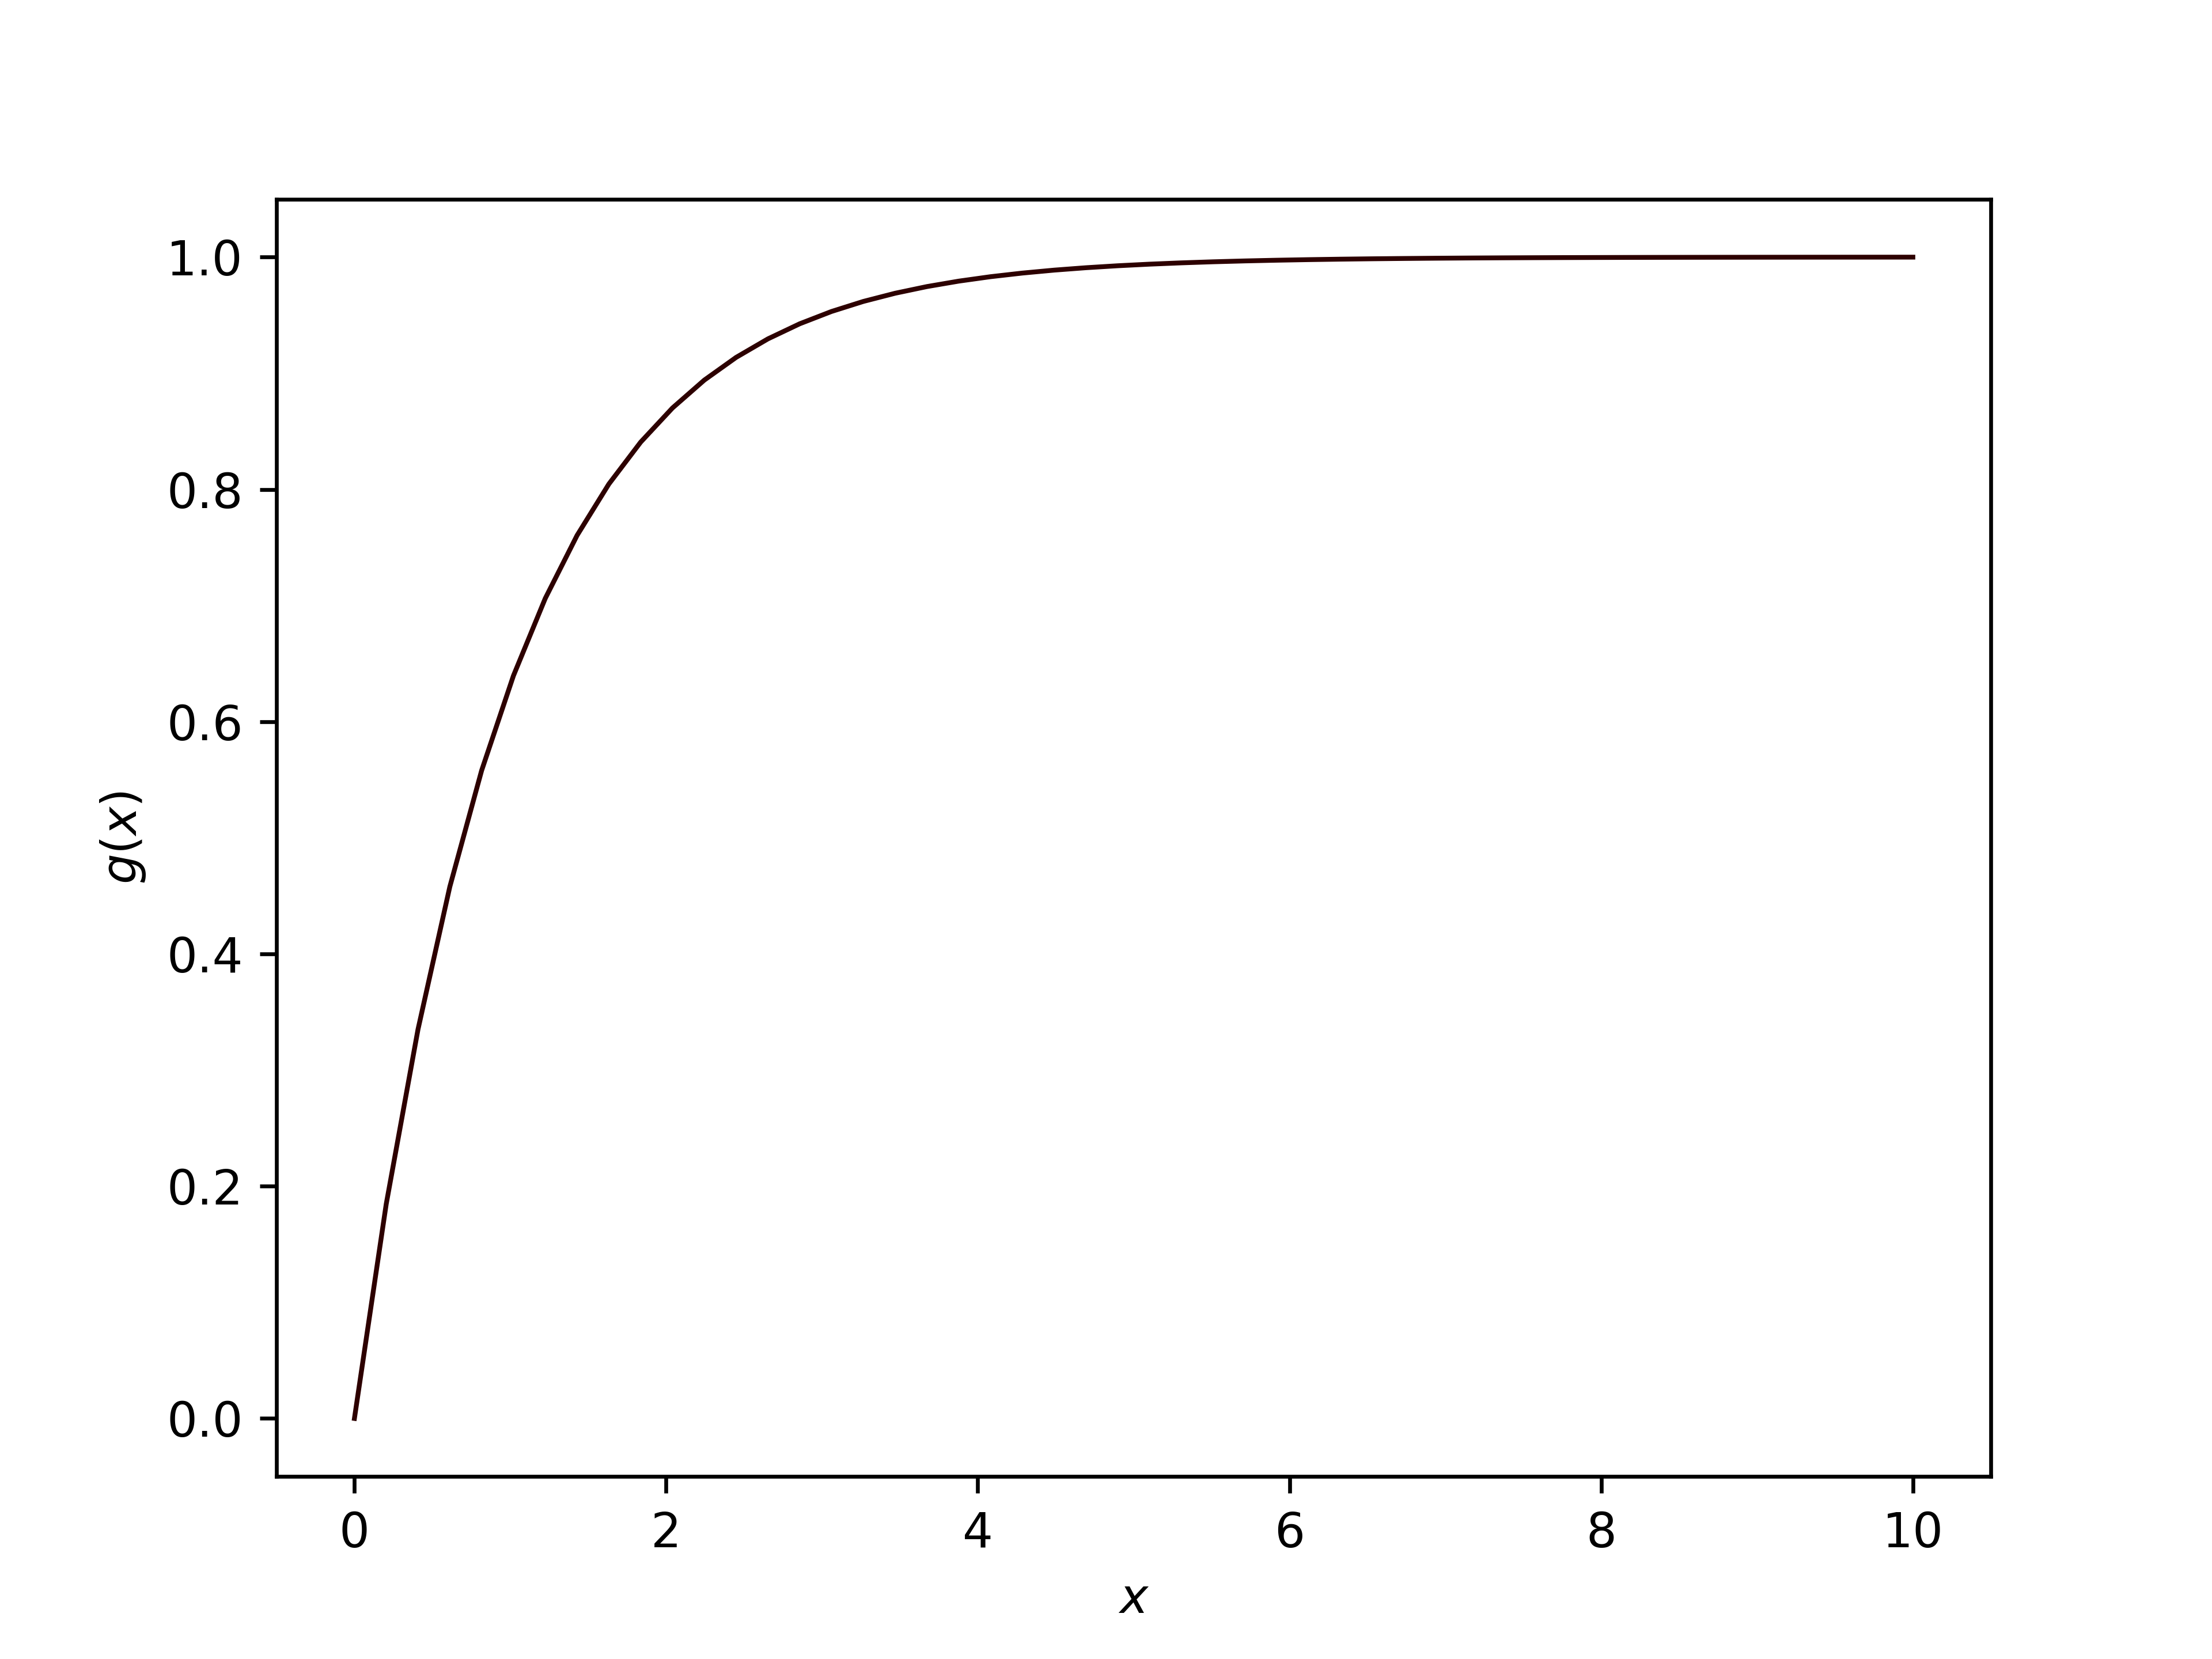
\includegraphics[width=0.8\textwidth]{figures/4_Functions/QQ3d.png}
\end{figure}

4.

Equilibrium acheived when $P^s = P^d$:

$$
  1+Q = a-bQ \implies Q(1+b) = a-1 \implies Q = \frac{a-1}{1+b}
$$

To be positive, either both numerator and denominator are positive, or both are negative:

$$
  (a>1 \land b>-1) \lor (a<1 \land b<-1)
$$


5.

a)

$$
  g(\lambda z, \lambda t) = 2\lambda^3t^2z = \lambda^3g(z, t) \therefore \text{homogeneous of degree 3.}
$$

b)

$$
  h(\lambda a, \lambda b) = \left( \lambda^2a^2+\lambda^2b^2 \right)^{\frac{1}{3}} = \lambda^{\frac{2}{3}}\left( a^2+b^2 \right)^{\frac{1}{3}} = \lambda^{\frac{2}{3}}h(a, b) \therefore \text{homogeneous of degree $\frac{2}{3}$.}
$$

\clearpage

\subsection{Long Questions}
\noindent

1.

a)

$$
  q^d(5) = 100\left( \frac{12}{5}-1 \right) = 140
$$

b)

$$
  q^d = 0 \implies \frac{12}{p} = 1 \implies p = 12
$$

c)

$$
  q^s = q^d \implies 50p = 100\left( \frac{12}{p}-1 \right) \implies p^2+2p-24 = 0 \implies (p+6)(p-4) = 0 \implies p = 4
$$

$$
  p=4 \implies q^s(4) = q^d(4) = 200
$$

d)

$$
  p^s(q) = \frac{q}{50}
$$

$$
  p^d(q): \quad \frac{12}{p} - 1 = \frac{q}{100} \implies \frac{12}{p} = \frac{q}{100} + 1 \implies p^d(q) = \frac{1200}{q+100}
$$

e)

$$
  \lim_{q\to\infty} p^d(q) = 0
$$

f)

\begin{figure}[H]
  \centering
  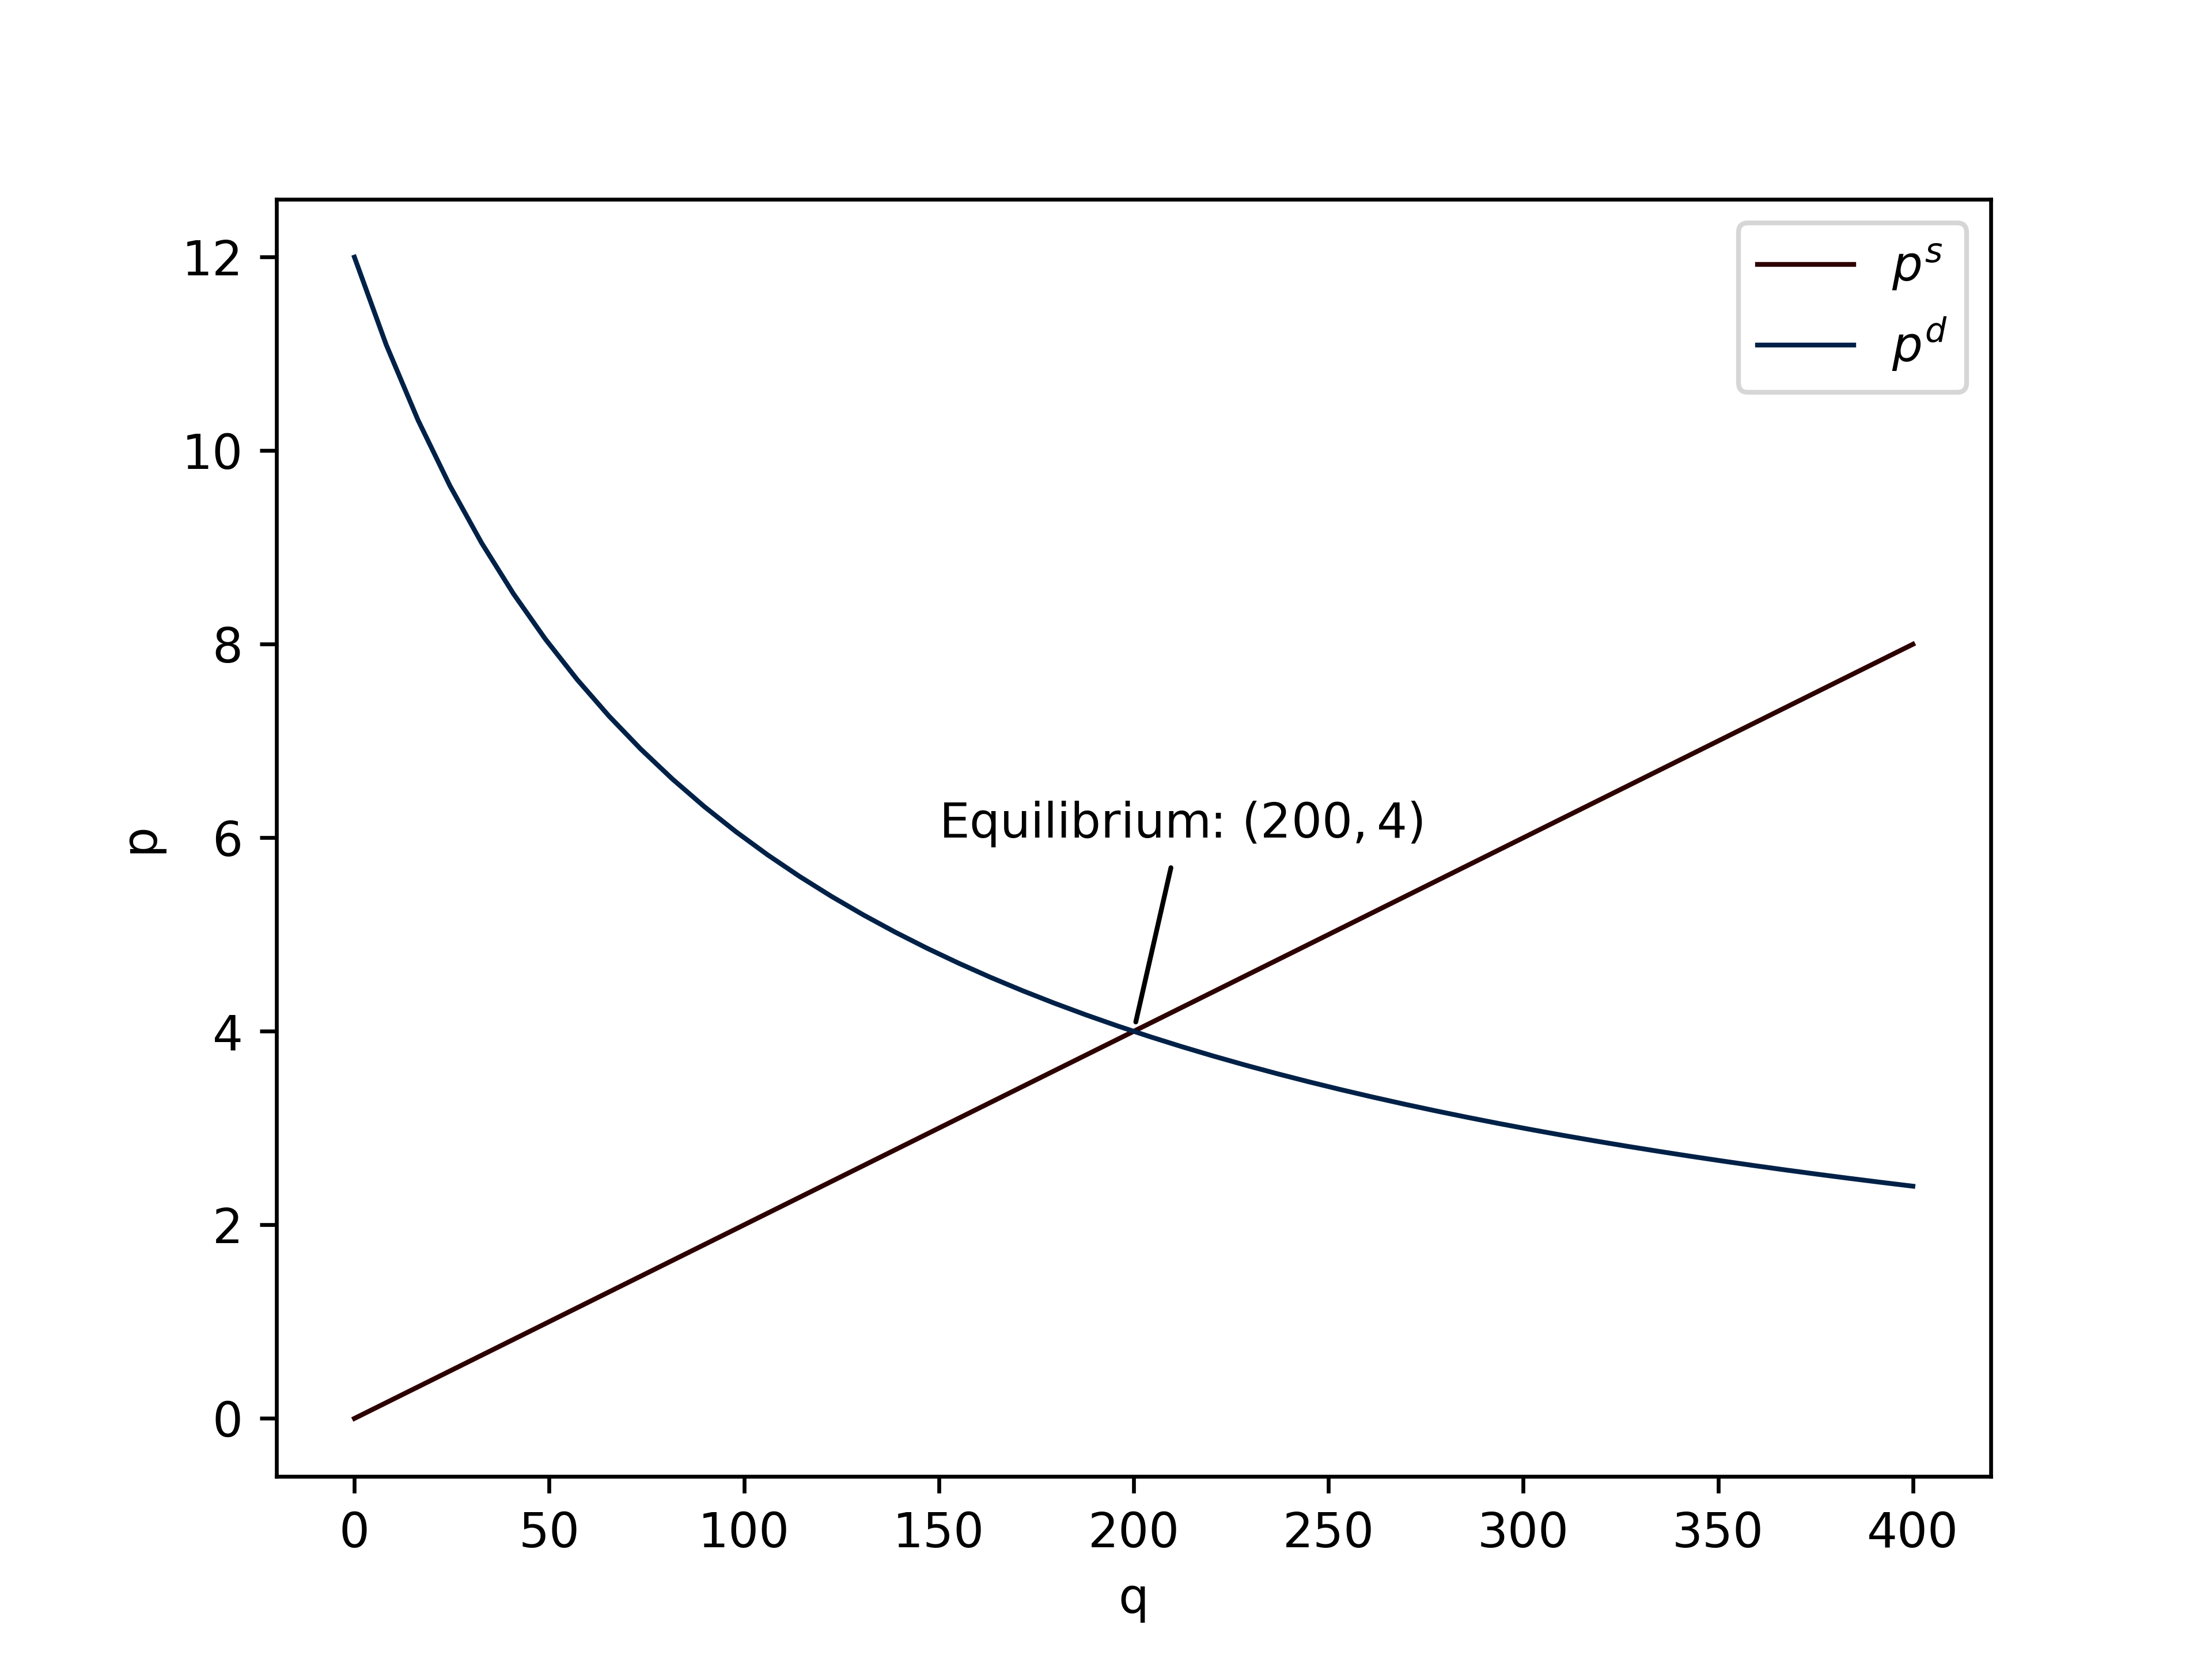
\includegraphics[width=0.8\textwidth]{figures/4_Functions/LQ1f.png}
\end{figure}

g)

\begin{figure}[H]
  \centering
  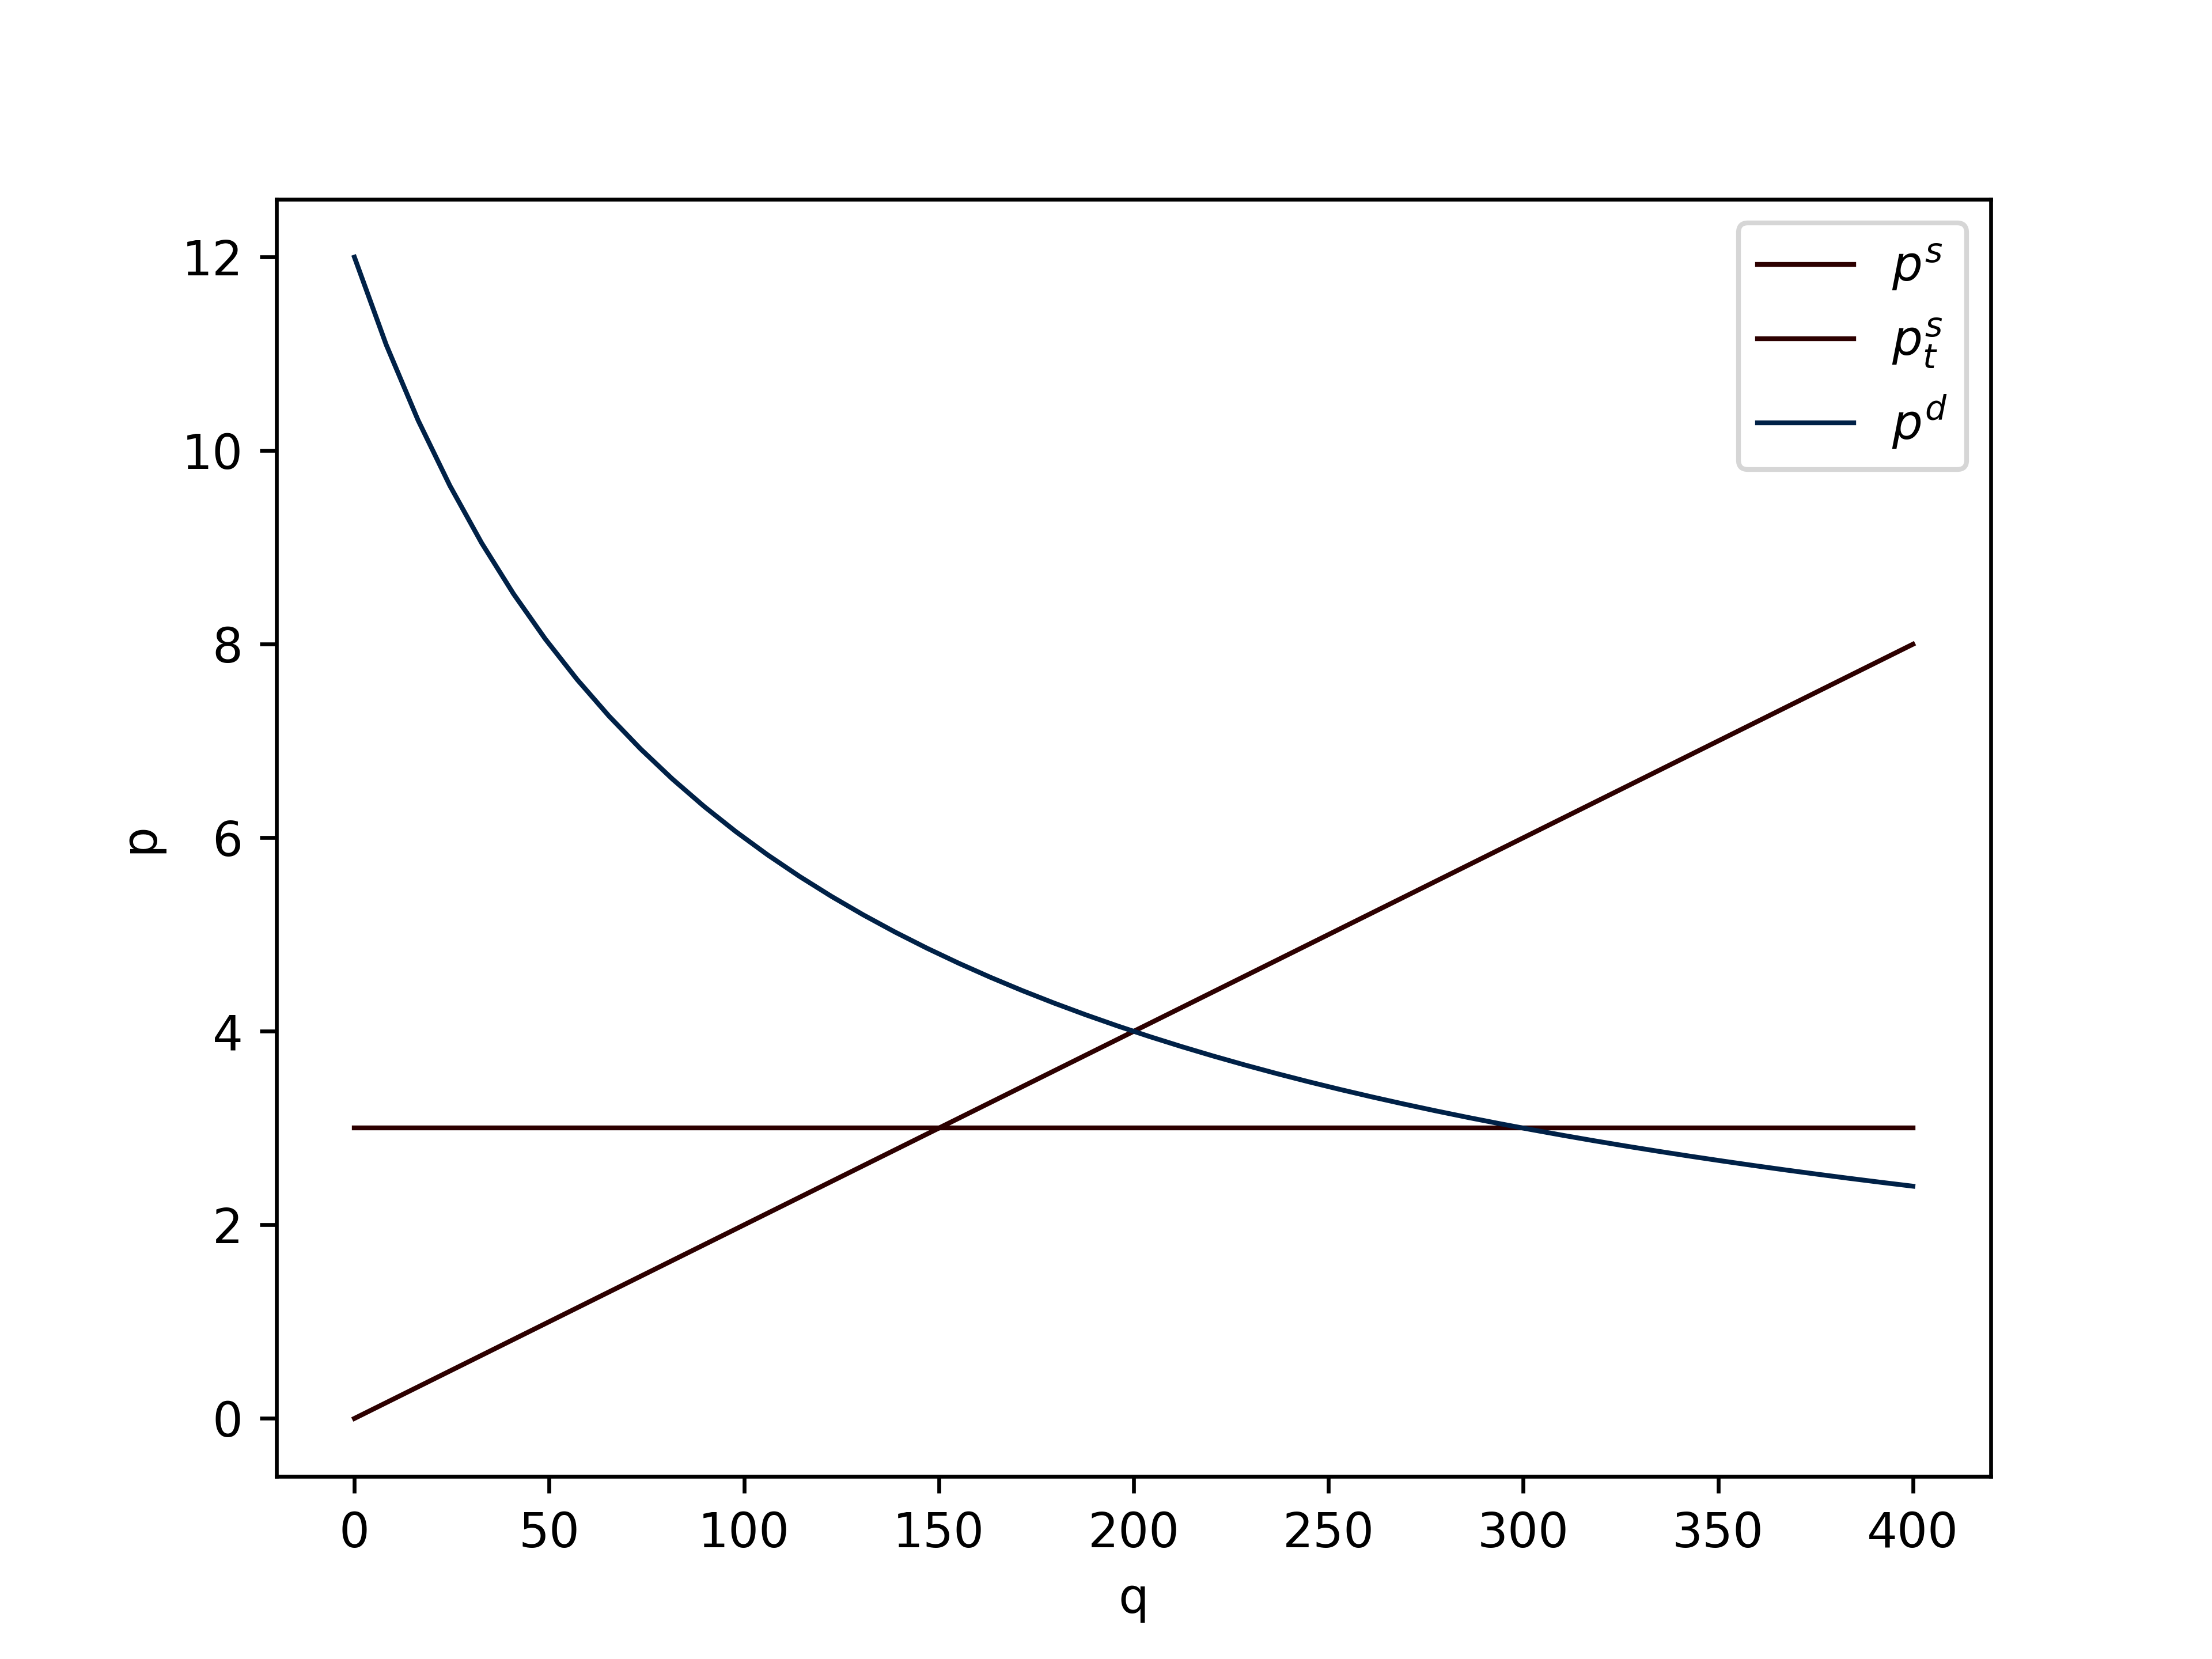
\includegraphics[width=0.8\textwidth]{figures/4_Functions/LQ1g.png}
\end{figure}

h)

$$
  1+t = \frac{1200}{q_e+100} \implies q_e+100 = \frac{1200}{1+t} \implies q_e = \frac{1200}{1+t} - 100
$$

$$
  p(q_e) = 1+t
$$

i)

Total taxed raised is $T=qt:$

$$
  T=qt = \frac{1200t}{1+t} - 100t
$$

\begin{figure}[H]
  \centering
  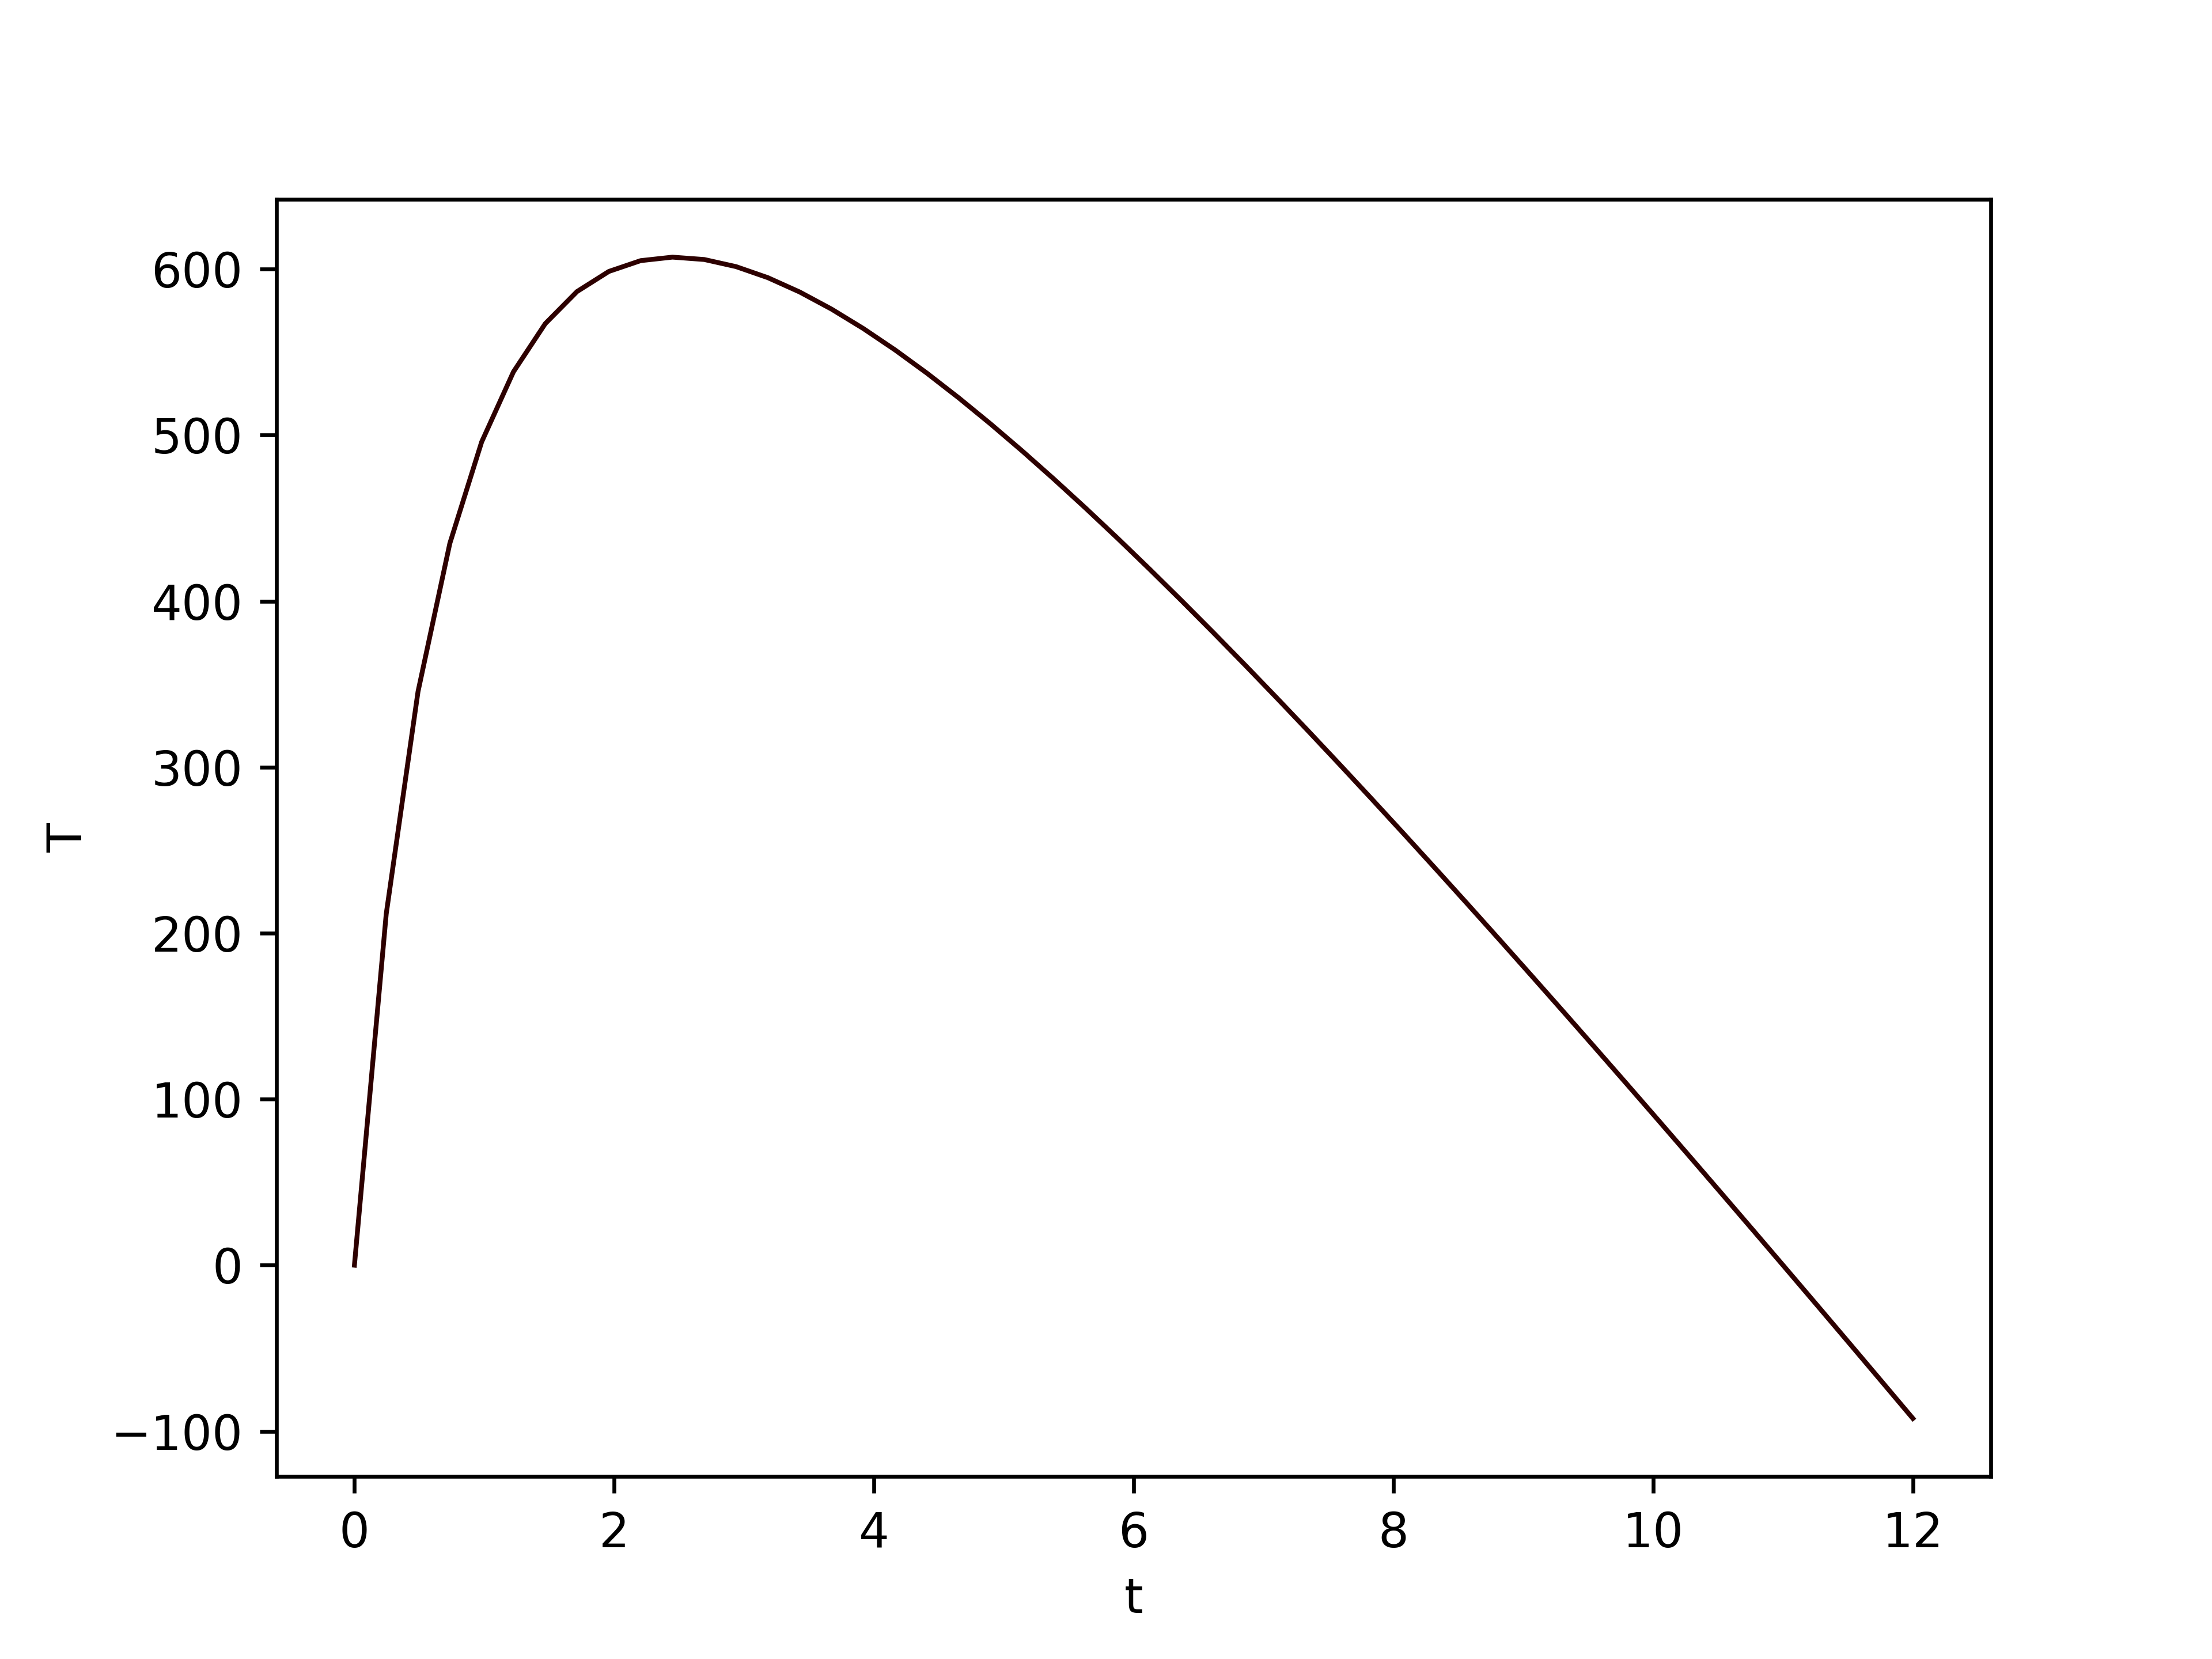
\includegraphics[width=0.8\textwidth]{figures/4_Functions/LQ1i.png}
\end{figure}

2.

a)

$$
  Y(\lambda n, \lambda m) = \left( \lambda n - \frac{\lambda m}{4} \right)^{\frac{2}{3}}\lambda^{\frac{1}{3}}m^{\frac{1}{3}} = \lambda^{\frac{2}{3}}\lambda^{\frac{1}{3}}\left( n - \frac{m}{4} \right)^{\frac{2}{3}}m^{\frac{1}{3}} = \lambda Y(n, m) \therefore \, \text{homogenous of degree 1 - constant returns to scale.}
$$

b)

\quad\quad i)

$$
  y(n) = Y(n, 8) = 2(n-2)^{\frac{2}{3}}
$$

\quad\quad ii)

\begin{figure}[H]
  \centering
  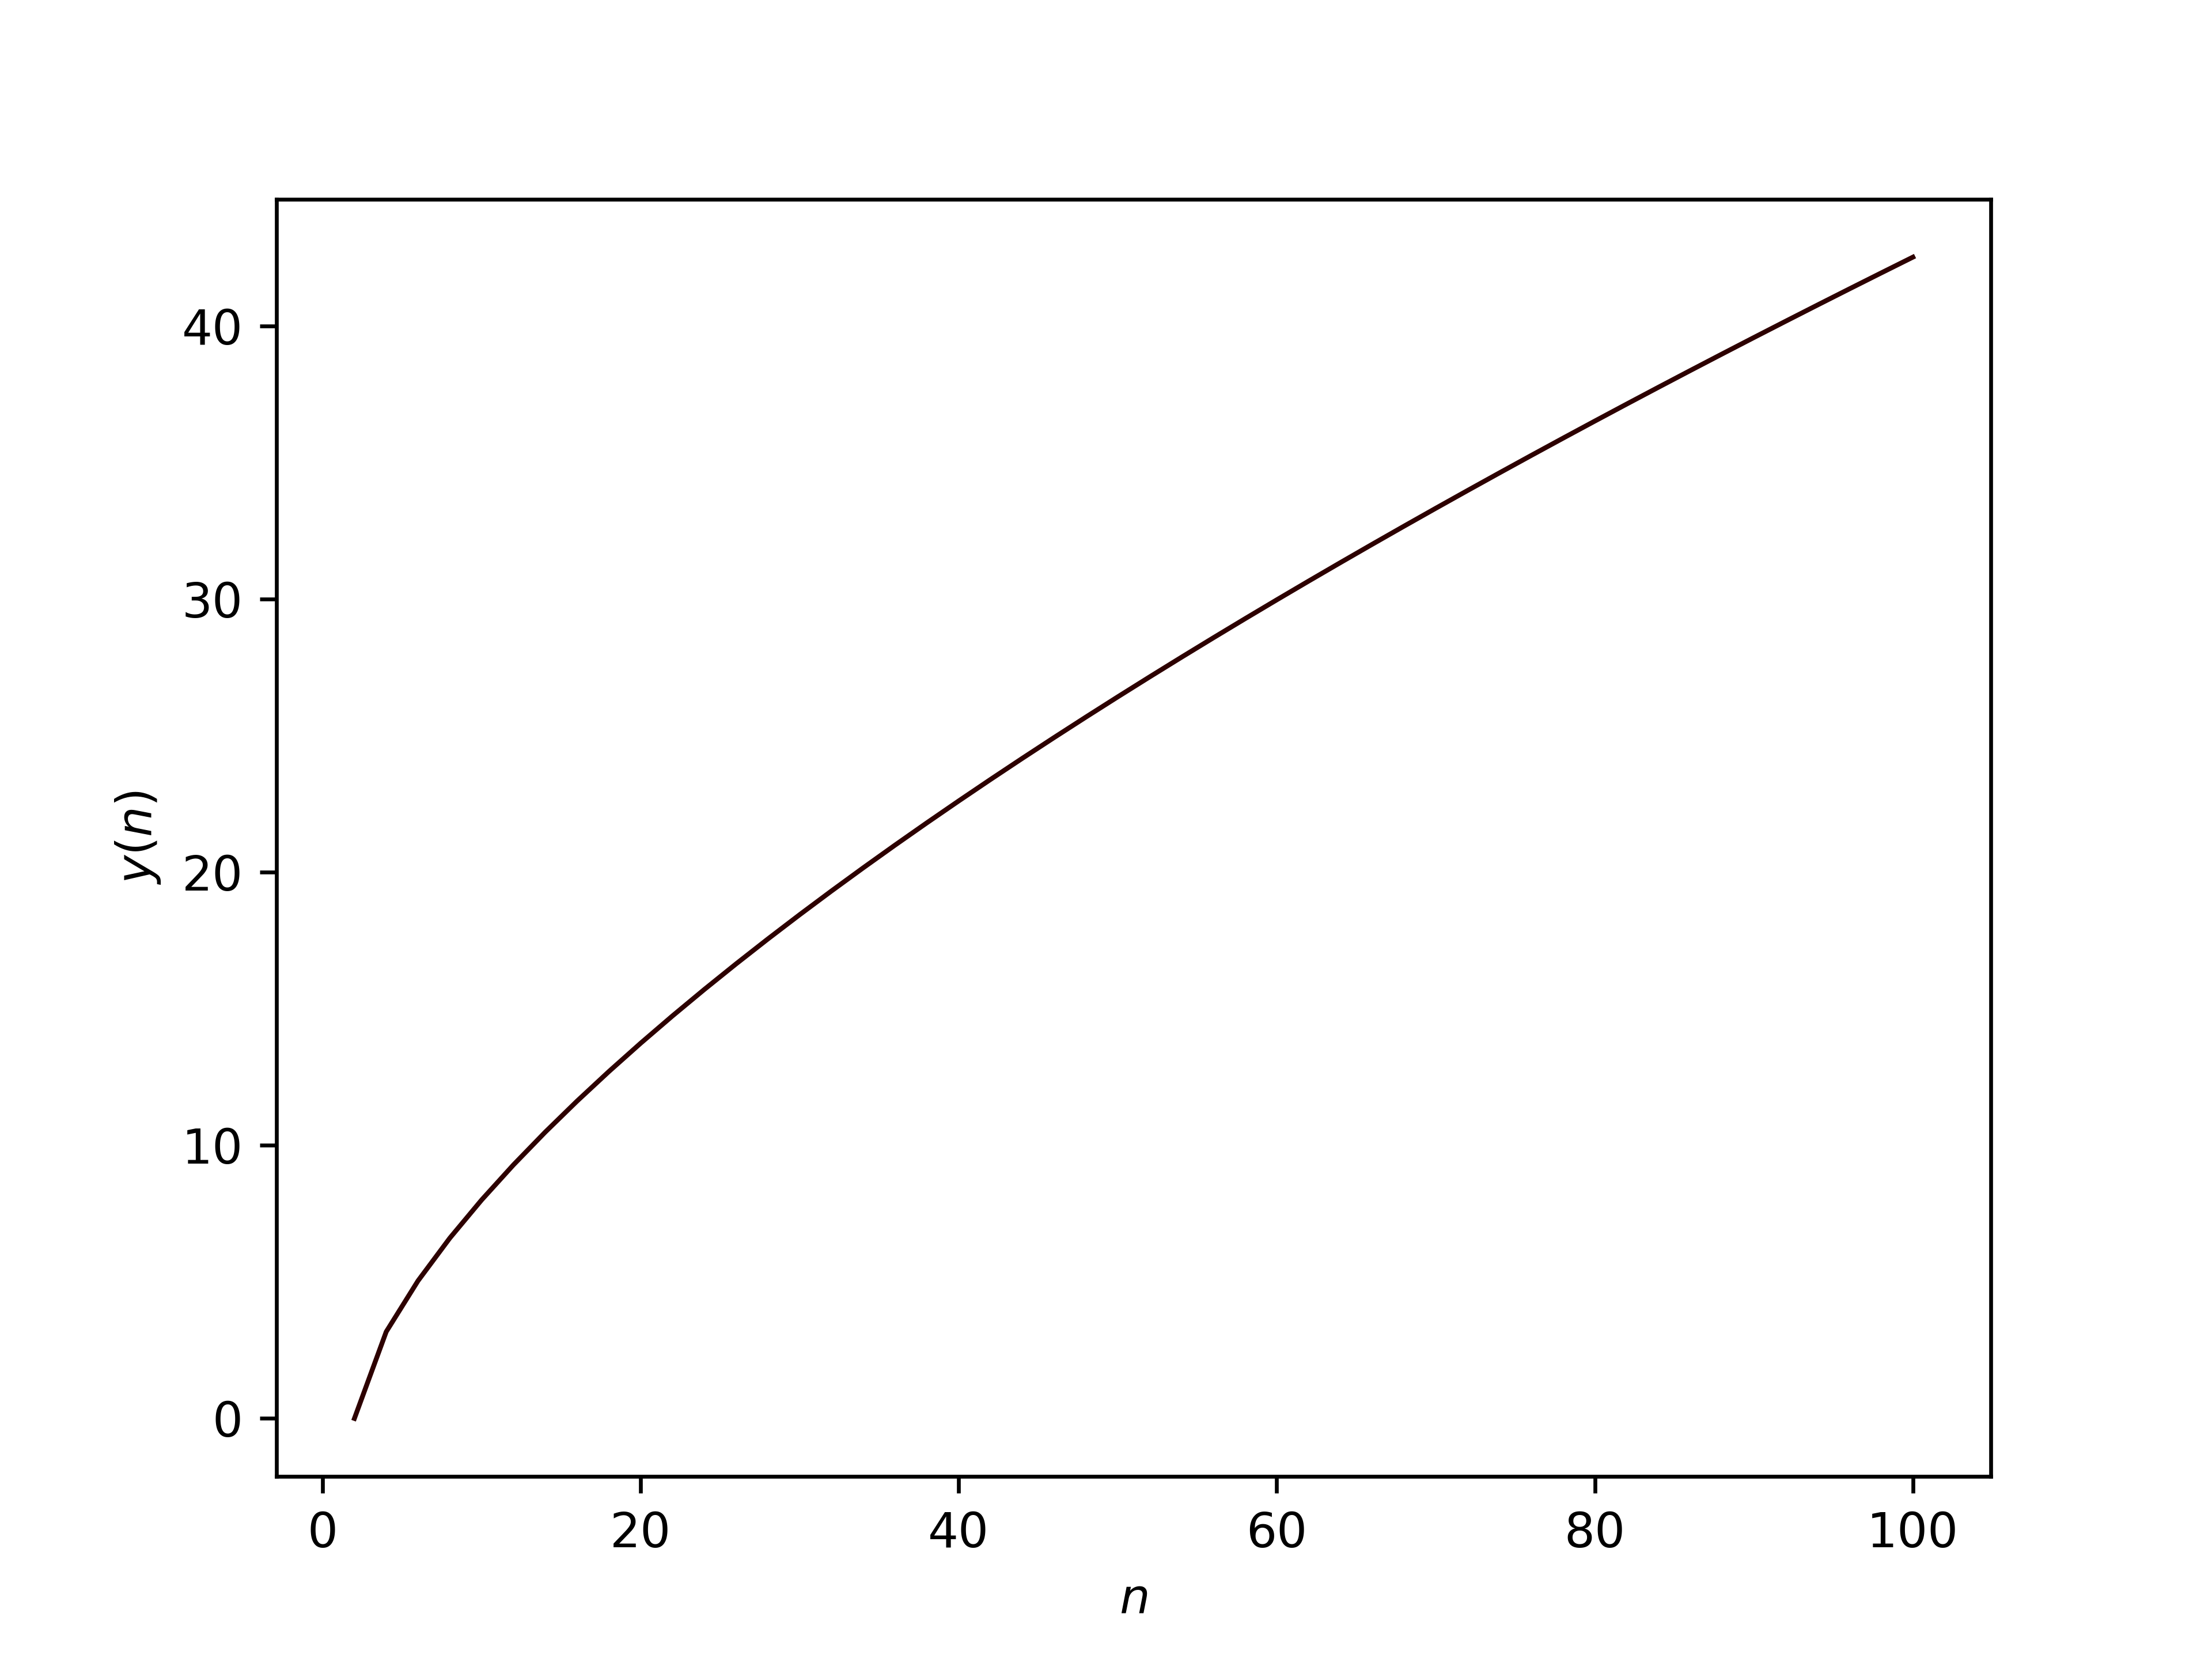
\includegraphics[width=0.8\textwidth]{figures/4_Functions/LQ2bii.png}
\end{figure}

Decreasing returns to labour.

\quad\quad iii)

$$
  \frac{y}{2} = (n-2)^{\frac{2}{3}} \implies n = 2 + \left( \frac{y}{2} \right)^{\frac{3}{2}}
$$

\begin{figure}[H]
  \centering
  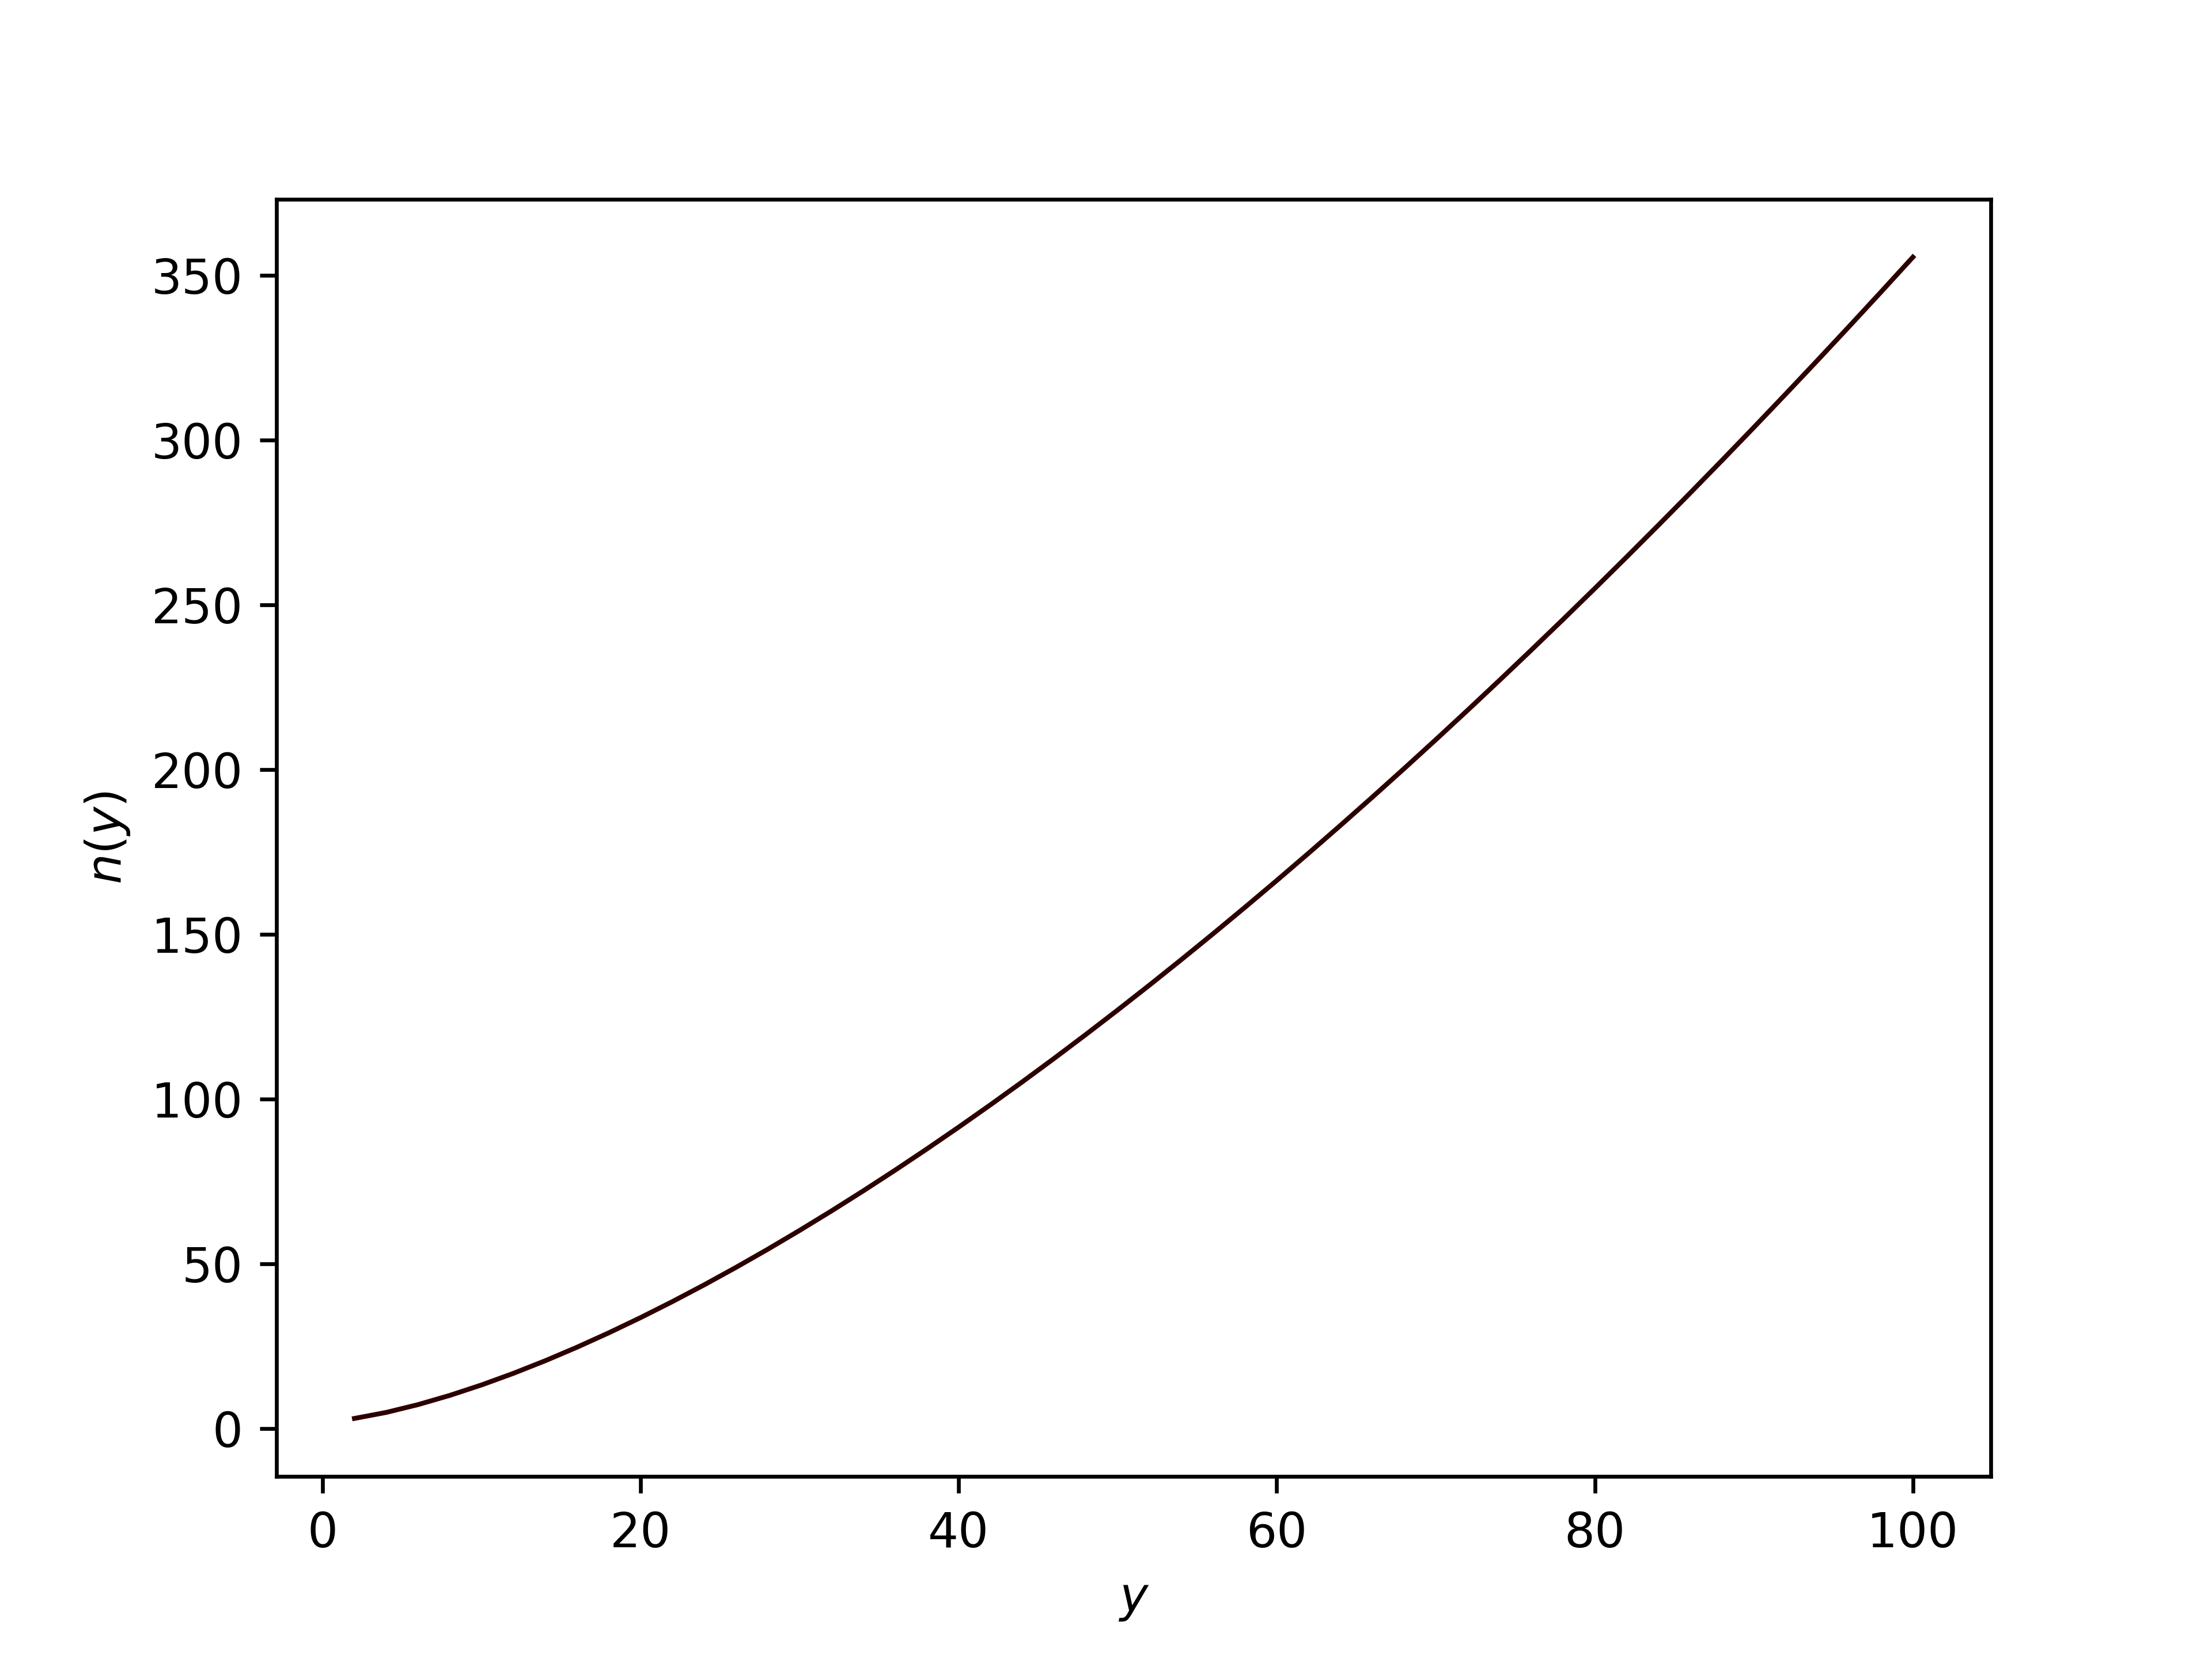
\includegraphics[width=0.8\textwidth]{figures/4_Functions/LQ2biii.png}
\end{figure}

$$
  n(16) = 2+8^{\frac{3}{2}}
$$

c)

\quad\quad i)

$$
  \left( n-\frac{m}{4} \right)^{\frac{2}{3}}m^{\frac{1}{3}} = 16 \implies \left( n-\frac{m}{4} \right)^2 = \frac{16}{m} \implies n = \frac{m}{4} + \sqrt{\frac{16}{m}}
$$

\begin{figure}[H]
  \centering
  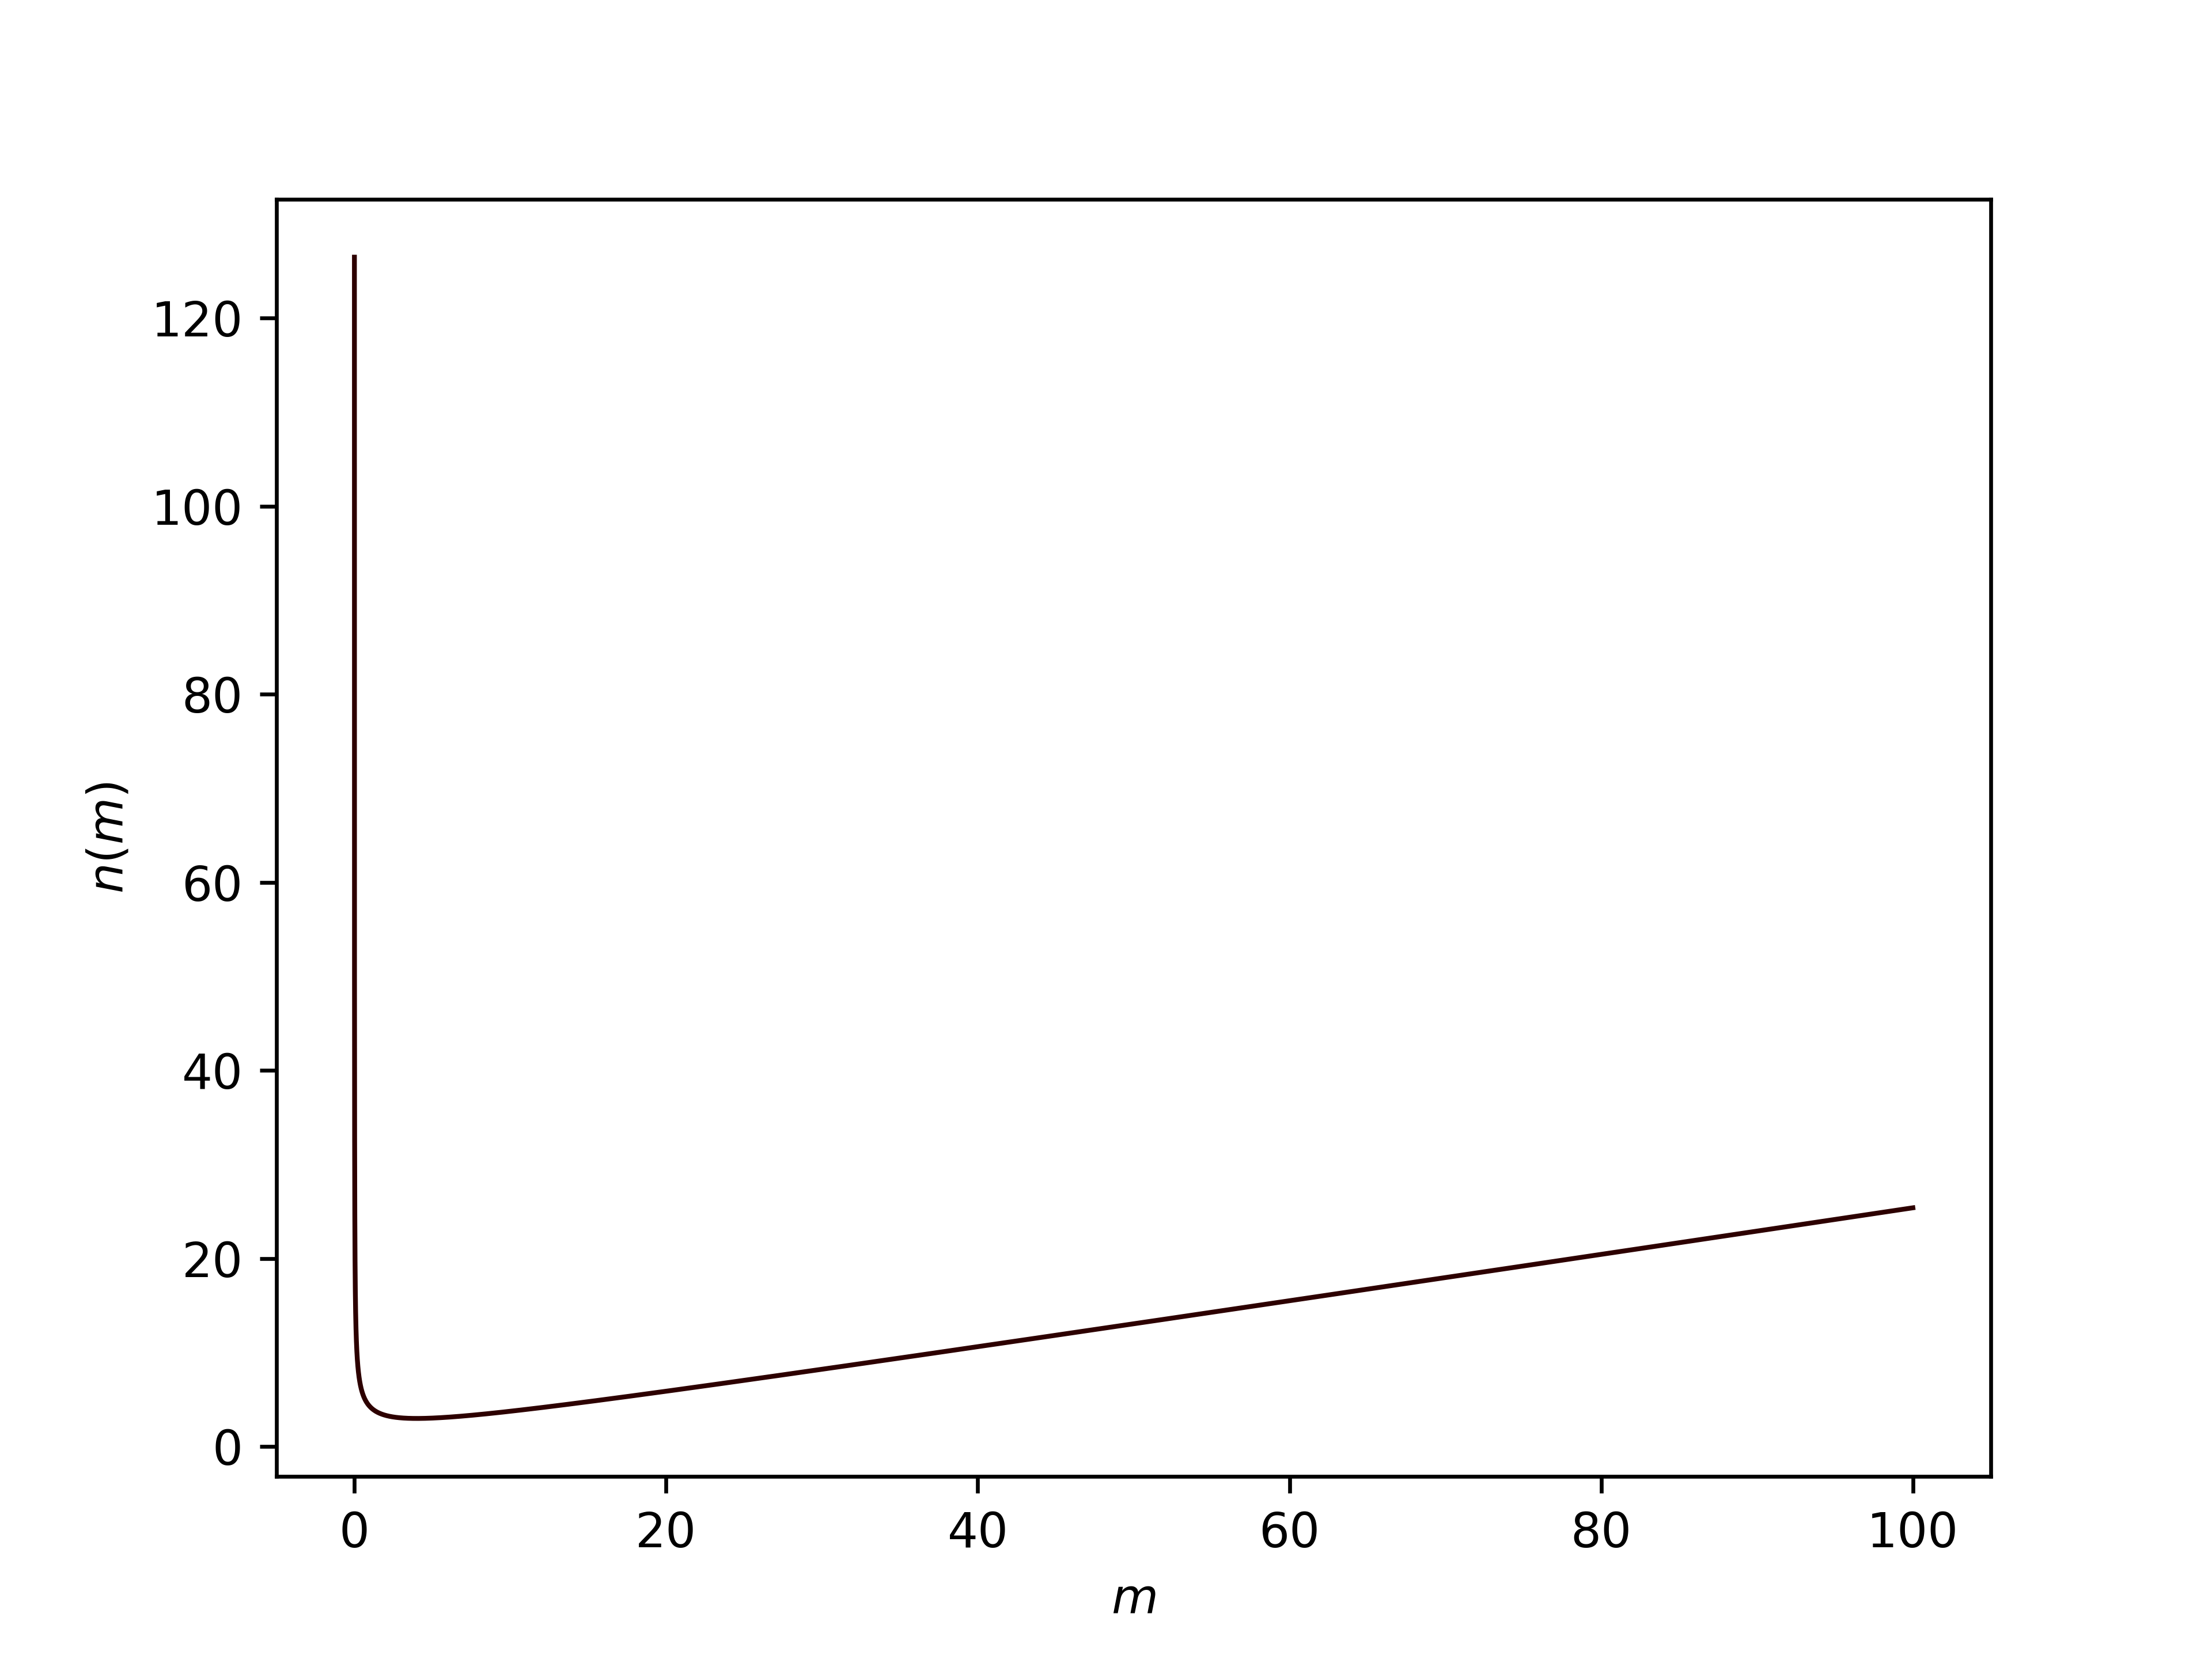
\includegraphics[width=0.8\textwidth]{figures/4_Functions/LQ2ci.png}
\end{figure}

As m increases, n must also increase in order to maintain the same output. Hence it would not be sensible to invest in a large number of machines, as the same output could be acheived with fewer machines, and fewer workers.

\clearpage

\section{Differentiation}

\subsection{Quick Questions}

\noindent

1.

\begin{center}
  \begin{tabular}{c}
    a) $\frac{\dd y}{\dd x} = 27x^2 - 14x$ \\
    b) $\frac{\dd f}{\dd x} = -\frac{3}{2x^3}$ \\
    c) $\frac{\dd Y}{\dd t} = 130t^{0.3}$ \\
    d) $\frac{\dd P}{\dd Q} = 2(Q - Q^{-\frac{1}{2}})$
  \end{tabular}
\end{center}

2.

\begin{center}
  \begin{tabular}{c}
    a) $y''(x) = 10 \geq 0 \quad \forall x \: \therefore \: \text{convex}$ \\
    b) $C''(y) = -\frac{1}{2y^{\frac{1}{2}}} \leq 0 \quad \forall y \geq 0 \: \therefore \: \text{concave}$ \\
    c) $P''(q) = 2 + \frac{1}{q^{\frac{3}{2}}} \geq 0 \quad \forall q \geq 0 \: \therefore \: \text{convex}$ \\
    d) $k''(x) = 2-6x \: \therefore \: \text{neither}$
  \end{tabular}
\end{center}

3.

$$
  F'(L) = 100 + \frac{400}{3}L^{-\frac{1}{3}}
$$

$$
  F''(L) = -\frac{400}{9}L^{-\frac{4}{3}}
$$

$$
  F''(L) \leq 0 \quad \forall L \geq 0 \: \therefore \: \text{diminishing returns to labour.}
$$

4.

a)

$$
  y = 3x - x^2 + 4 \implies \frac{\dd y}{\dd x} = 3-2x \overset{!}{=} 0 \implies x = \frac{3}{2}, \: y \left( \frac{3}{2} \right) = \frac{25}{4}
$$

$$
  y''(x) = -2 < 0 \: \therefore \: \text{maximum}
$$

\begin{figure}[H]
  \centering
  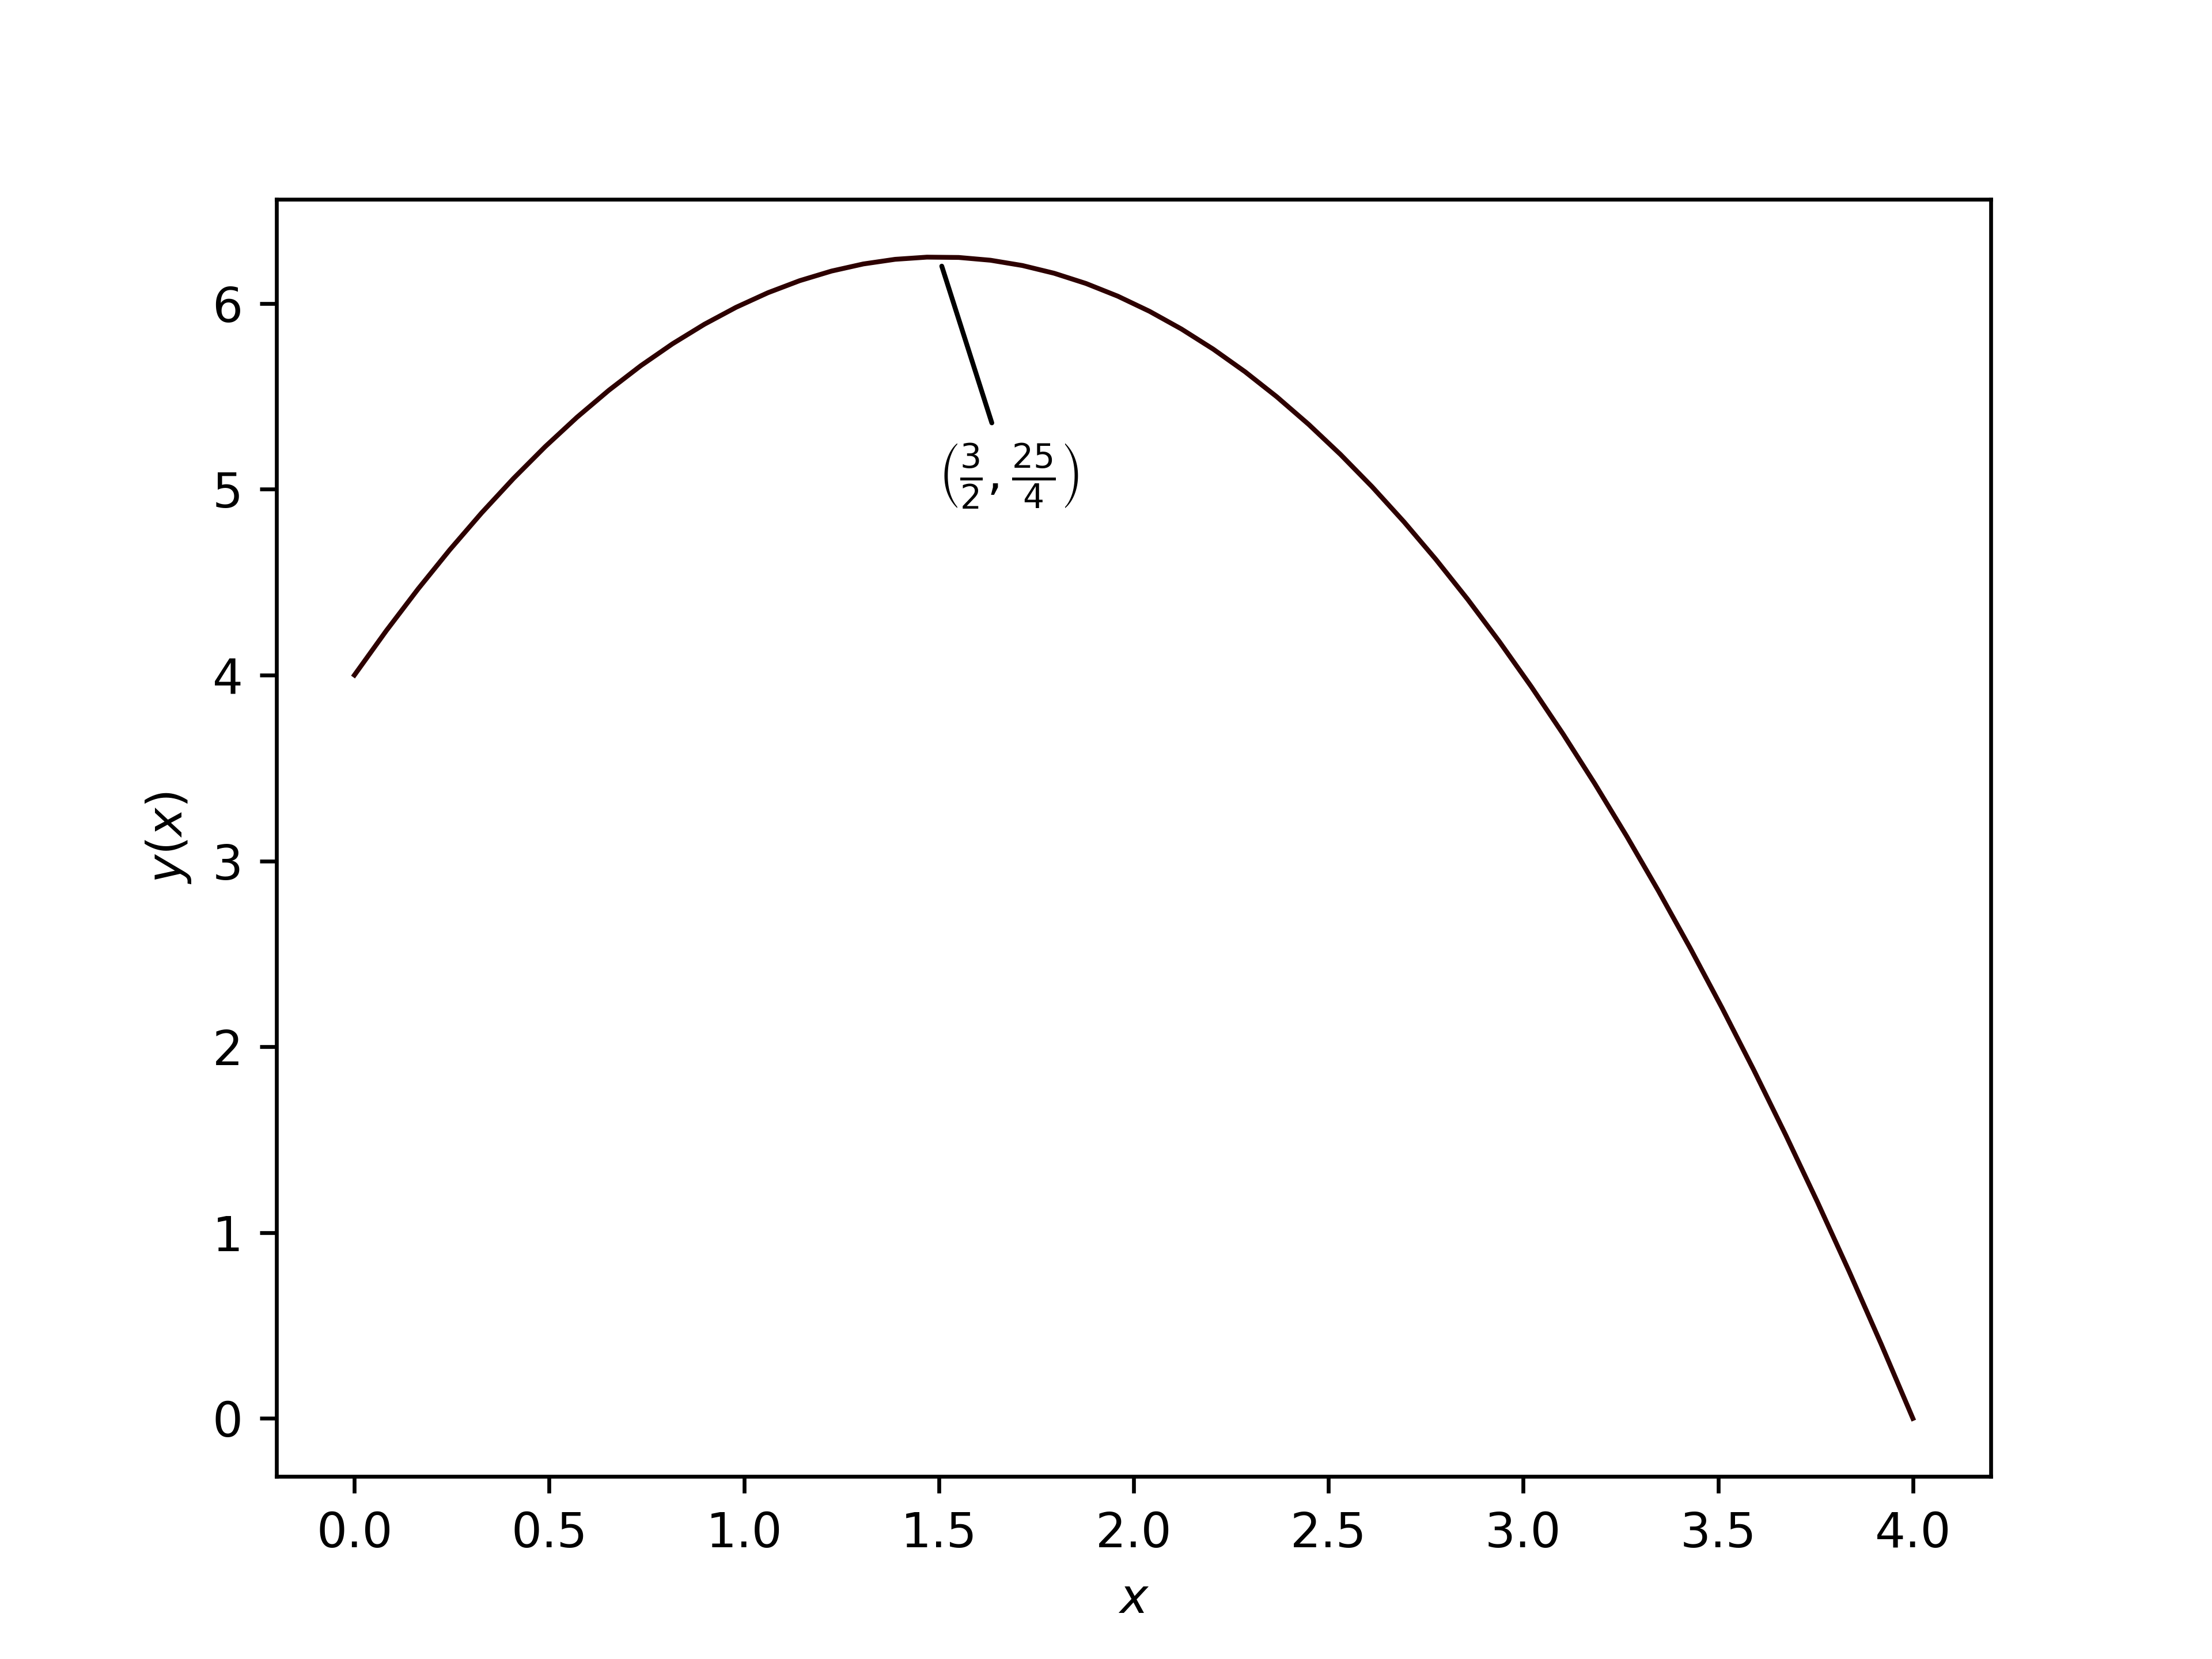
\includegraphics[width=0.8\textwidth]{figures/5_Differentiation/QQ4a.png}
\end{figure}

b)

$$
  g = 6x^{\frac{1}{2}} - x \implies \frac{\dd g}{\dd x} = 3x^{-\frac{1}{3}} - 1 \overset{!}{=} 0 \implies x^{\frac{1}{2}} = 3 \implies x = 9, \: g(9) = 9
$$

$$
  g''(9) = -\frac{3}{2} 9^{-\frac{3}{2}} = -\frac{3}{2}\cdot3^{-3} < 0 \: \therefore \: \text{maximum}
$$

\begin{figure}[H]
  \centering
  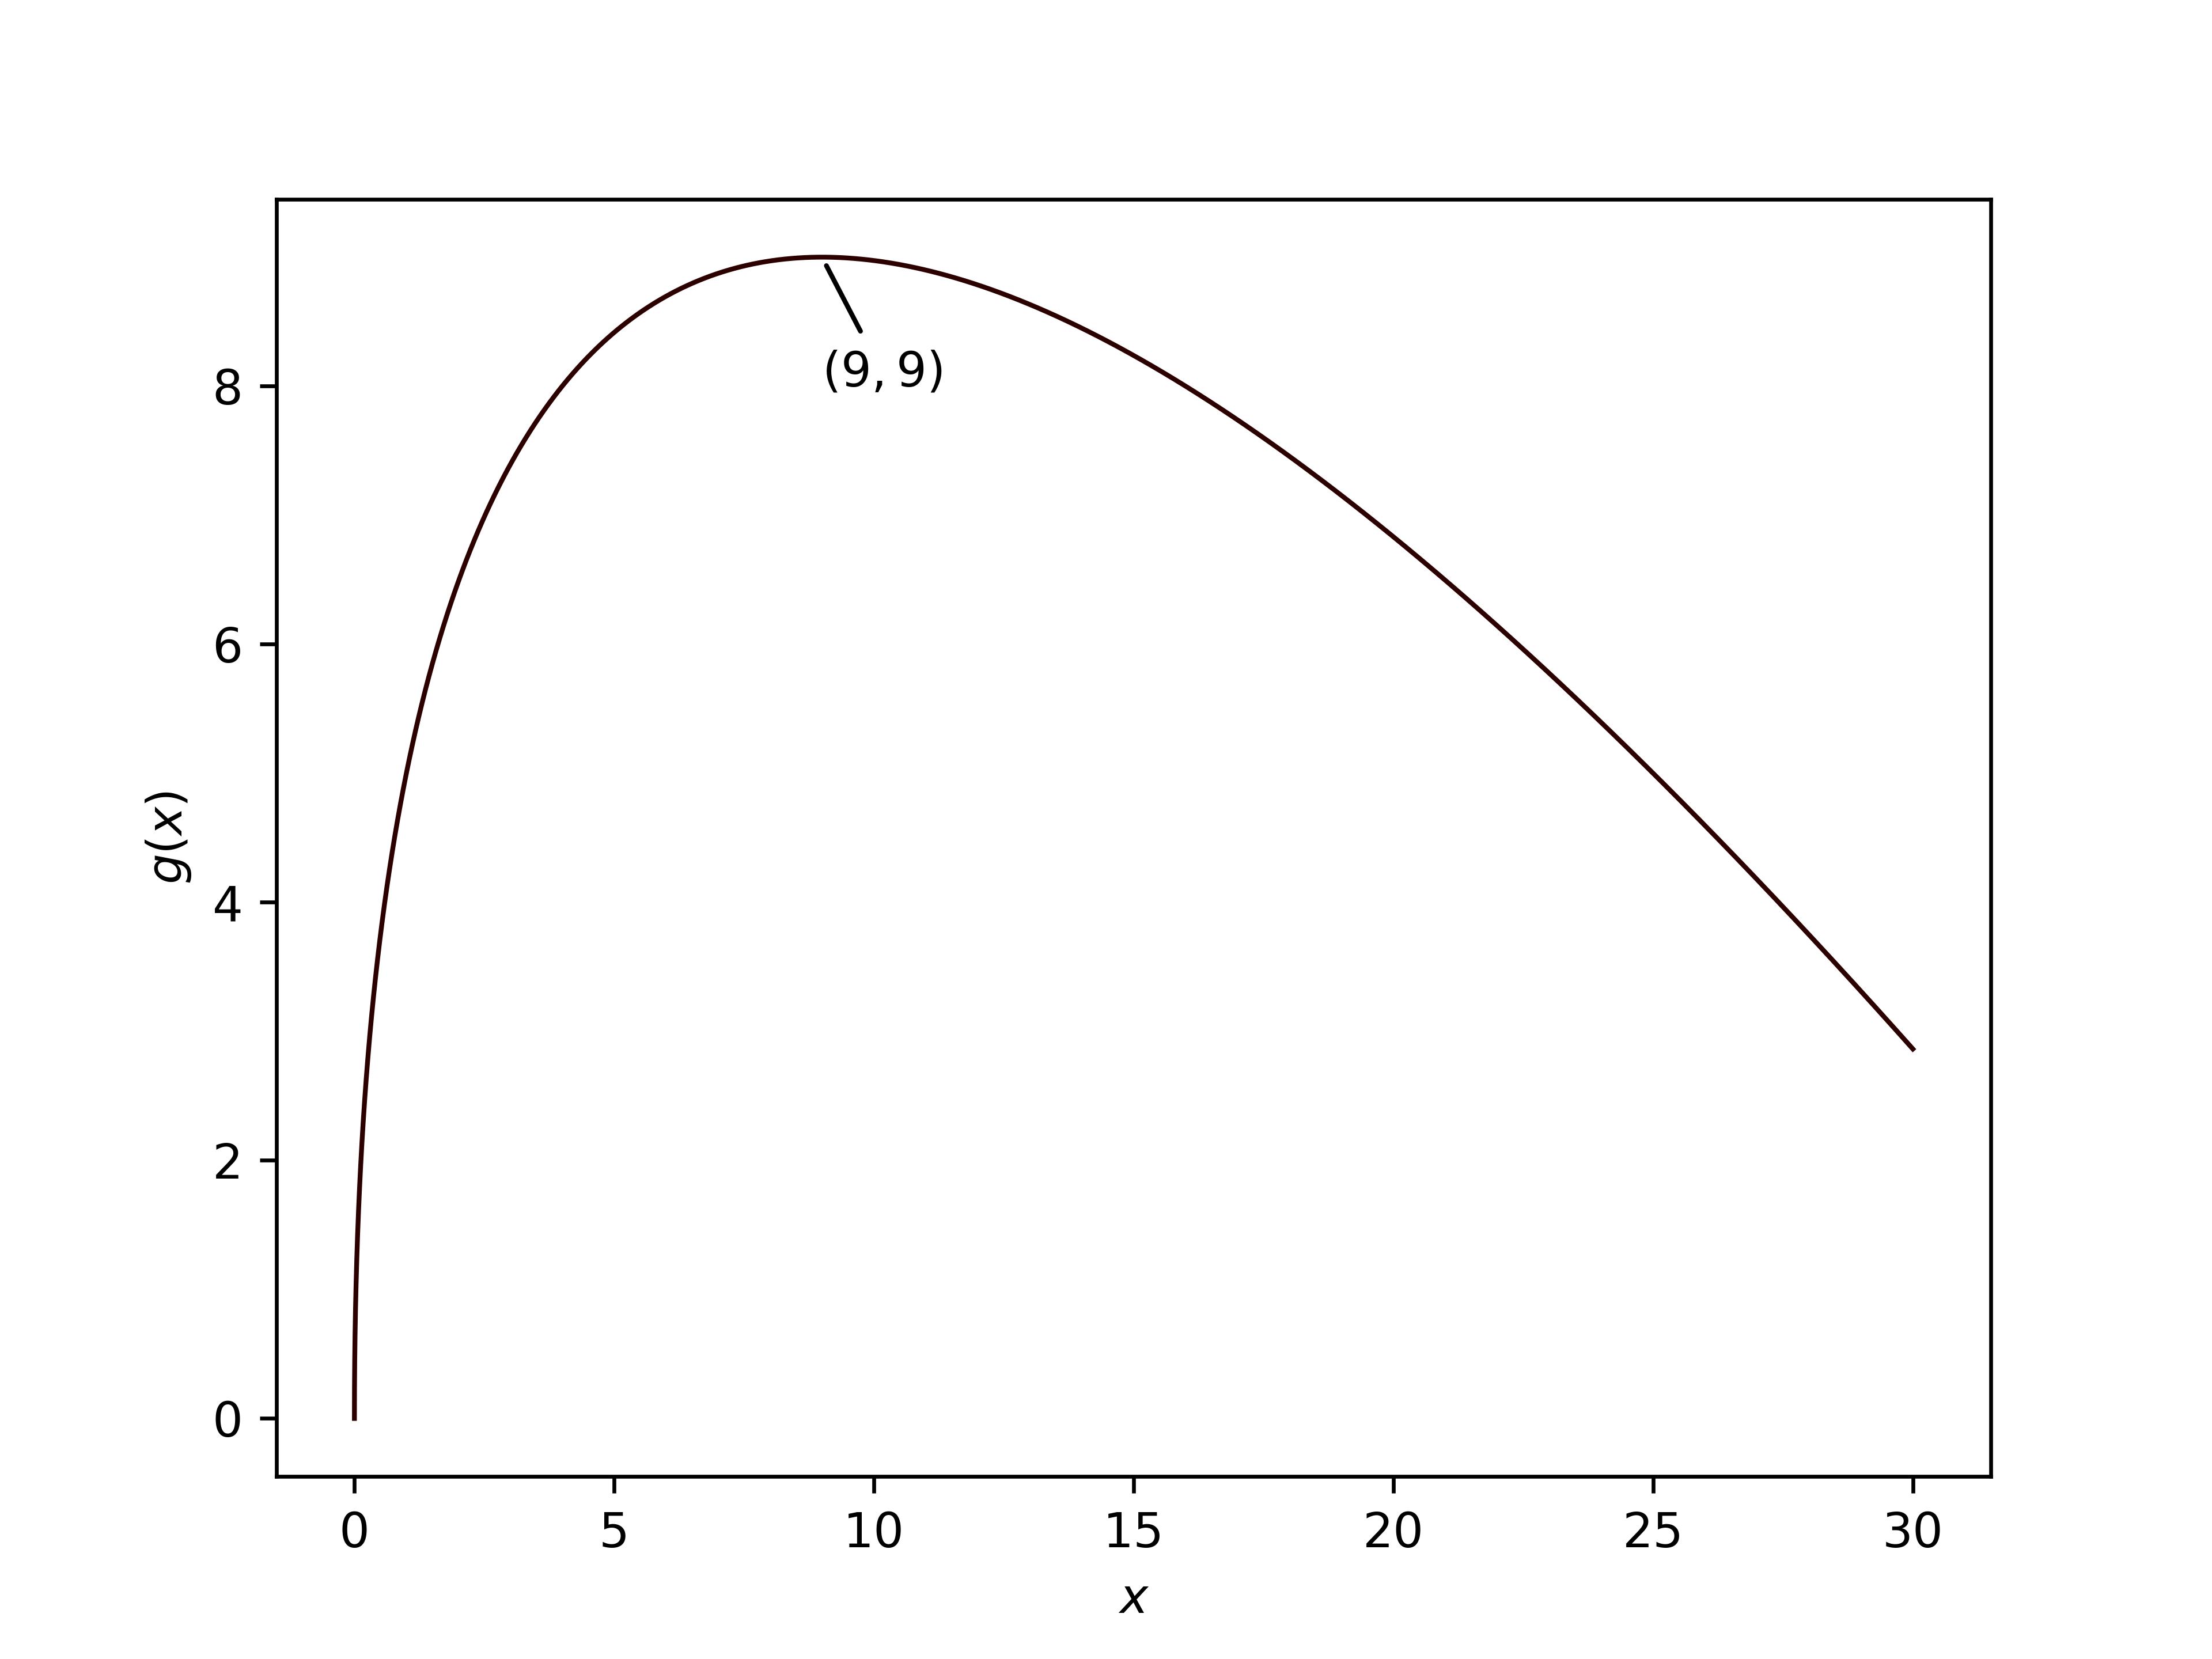
\includegraphics[width=0.8\textwidth]{figures/5_Differentiation/QQ4b.png}
\end{figure}

c)

$$
  f = x^4 - 8x^3 + 18x^2 -5 \implies \frac{\dd f}{\dd x} = 4x^3 - 24x^2 + 36x \overset{!}{=} 0 \implies x(x-3)^2 = 0 \implies x = 0, \: x = 3
$$

$$
  x = 0, \: f(0) = -5, \: f''(0) = 36 \: \therefore \: \text{minimum}
$$

$$
  x = 3, \: f(3) = 22, \: f''(3) = 0 \: \therefore \: \text{inflection}
$$

\begin{figure}[H]
  \centering
  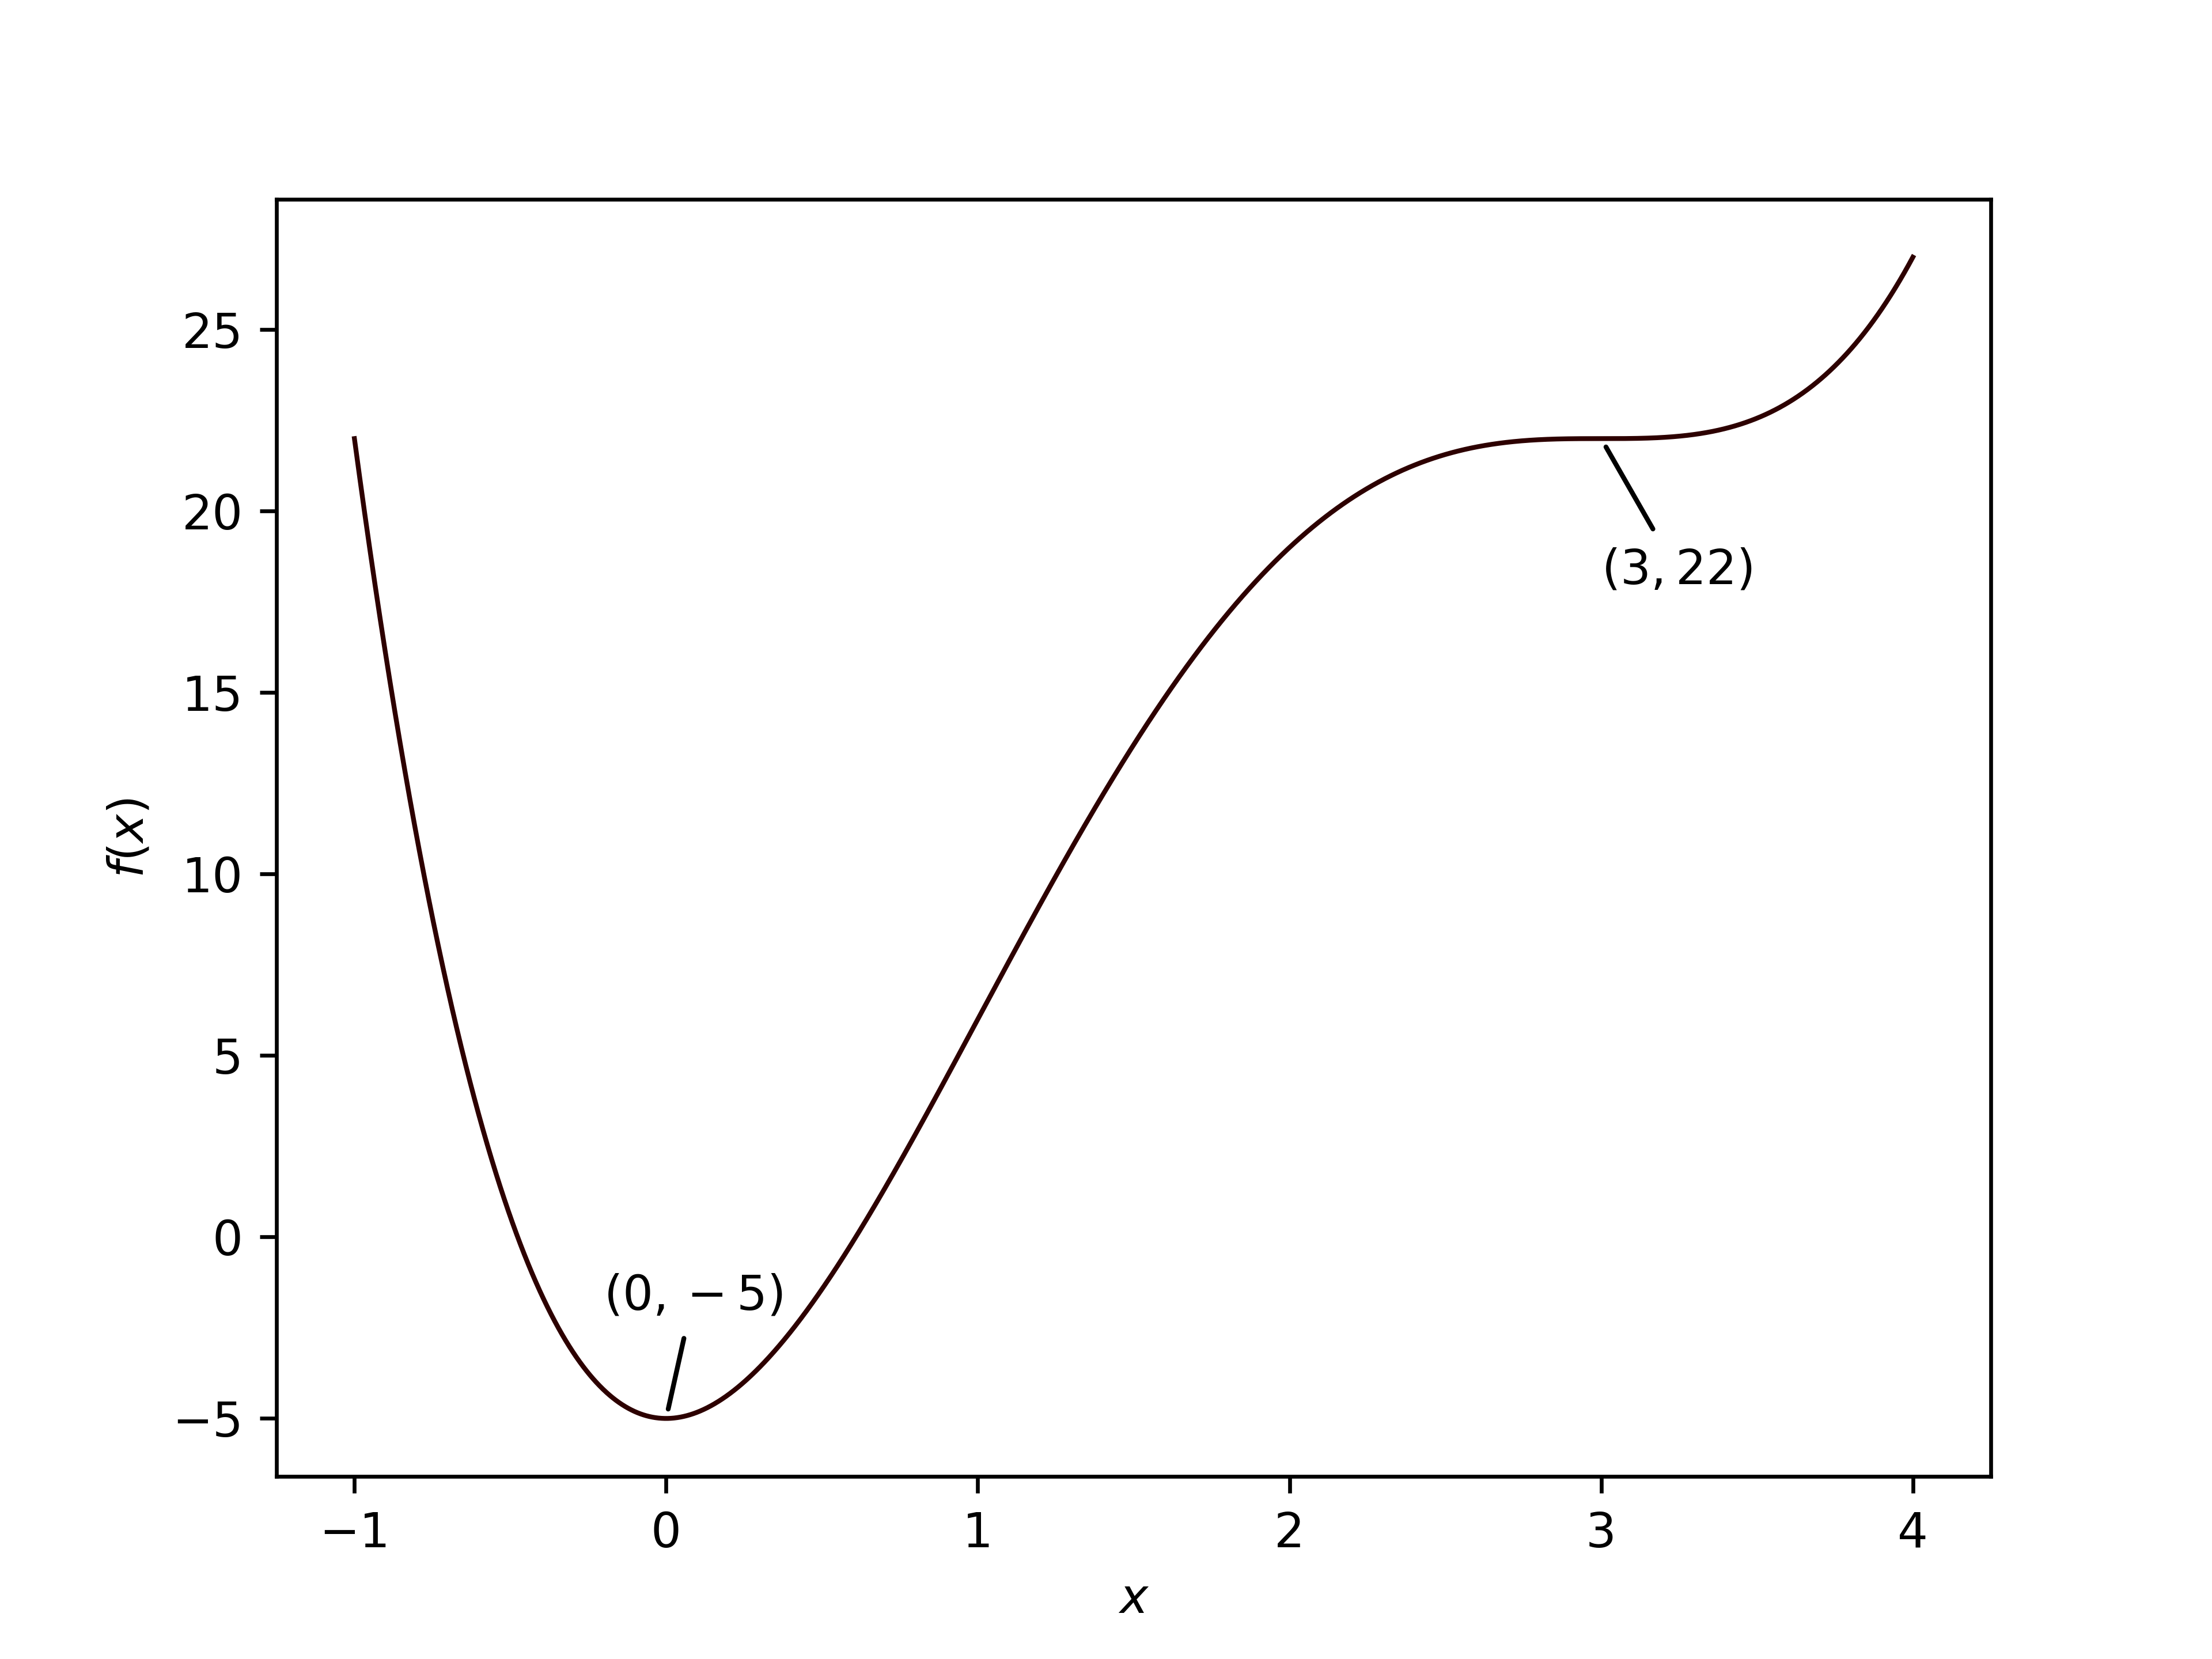
\includegraphics[width=0.8\textwidth]{figures/5_Differentiation/QQ4c.png}
\end{figure}


5.

$$
  MC(Q) = \frac{\dd C}{\dd Q} = a\left[ b+\frac{5}{2}Q^{\frac{3}{2}}  \right]
$$

\begin{figure}[H]
  \centering
  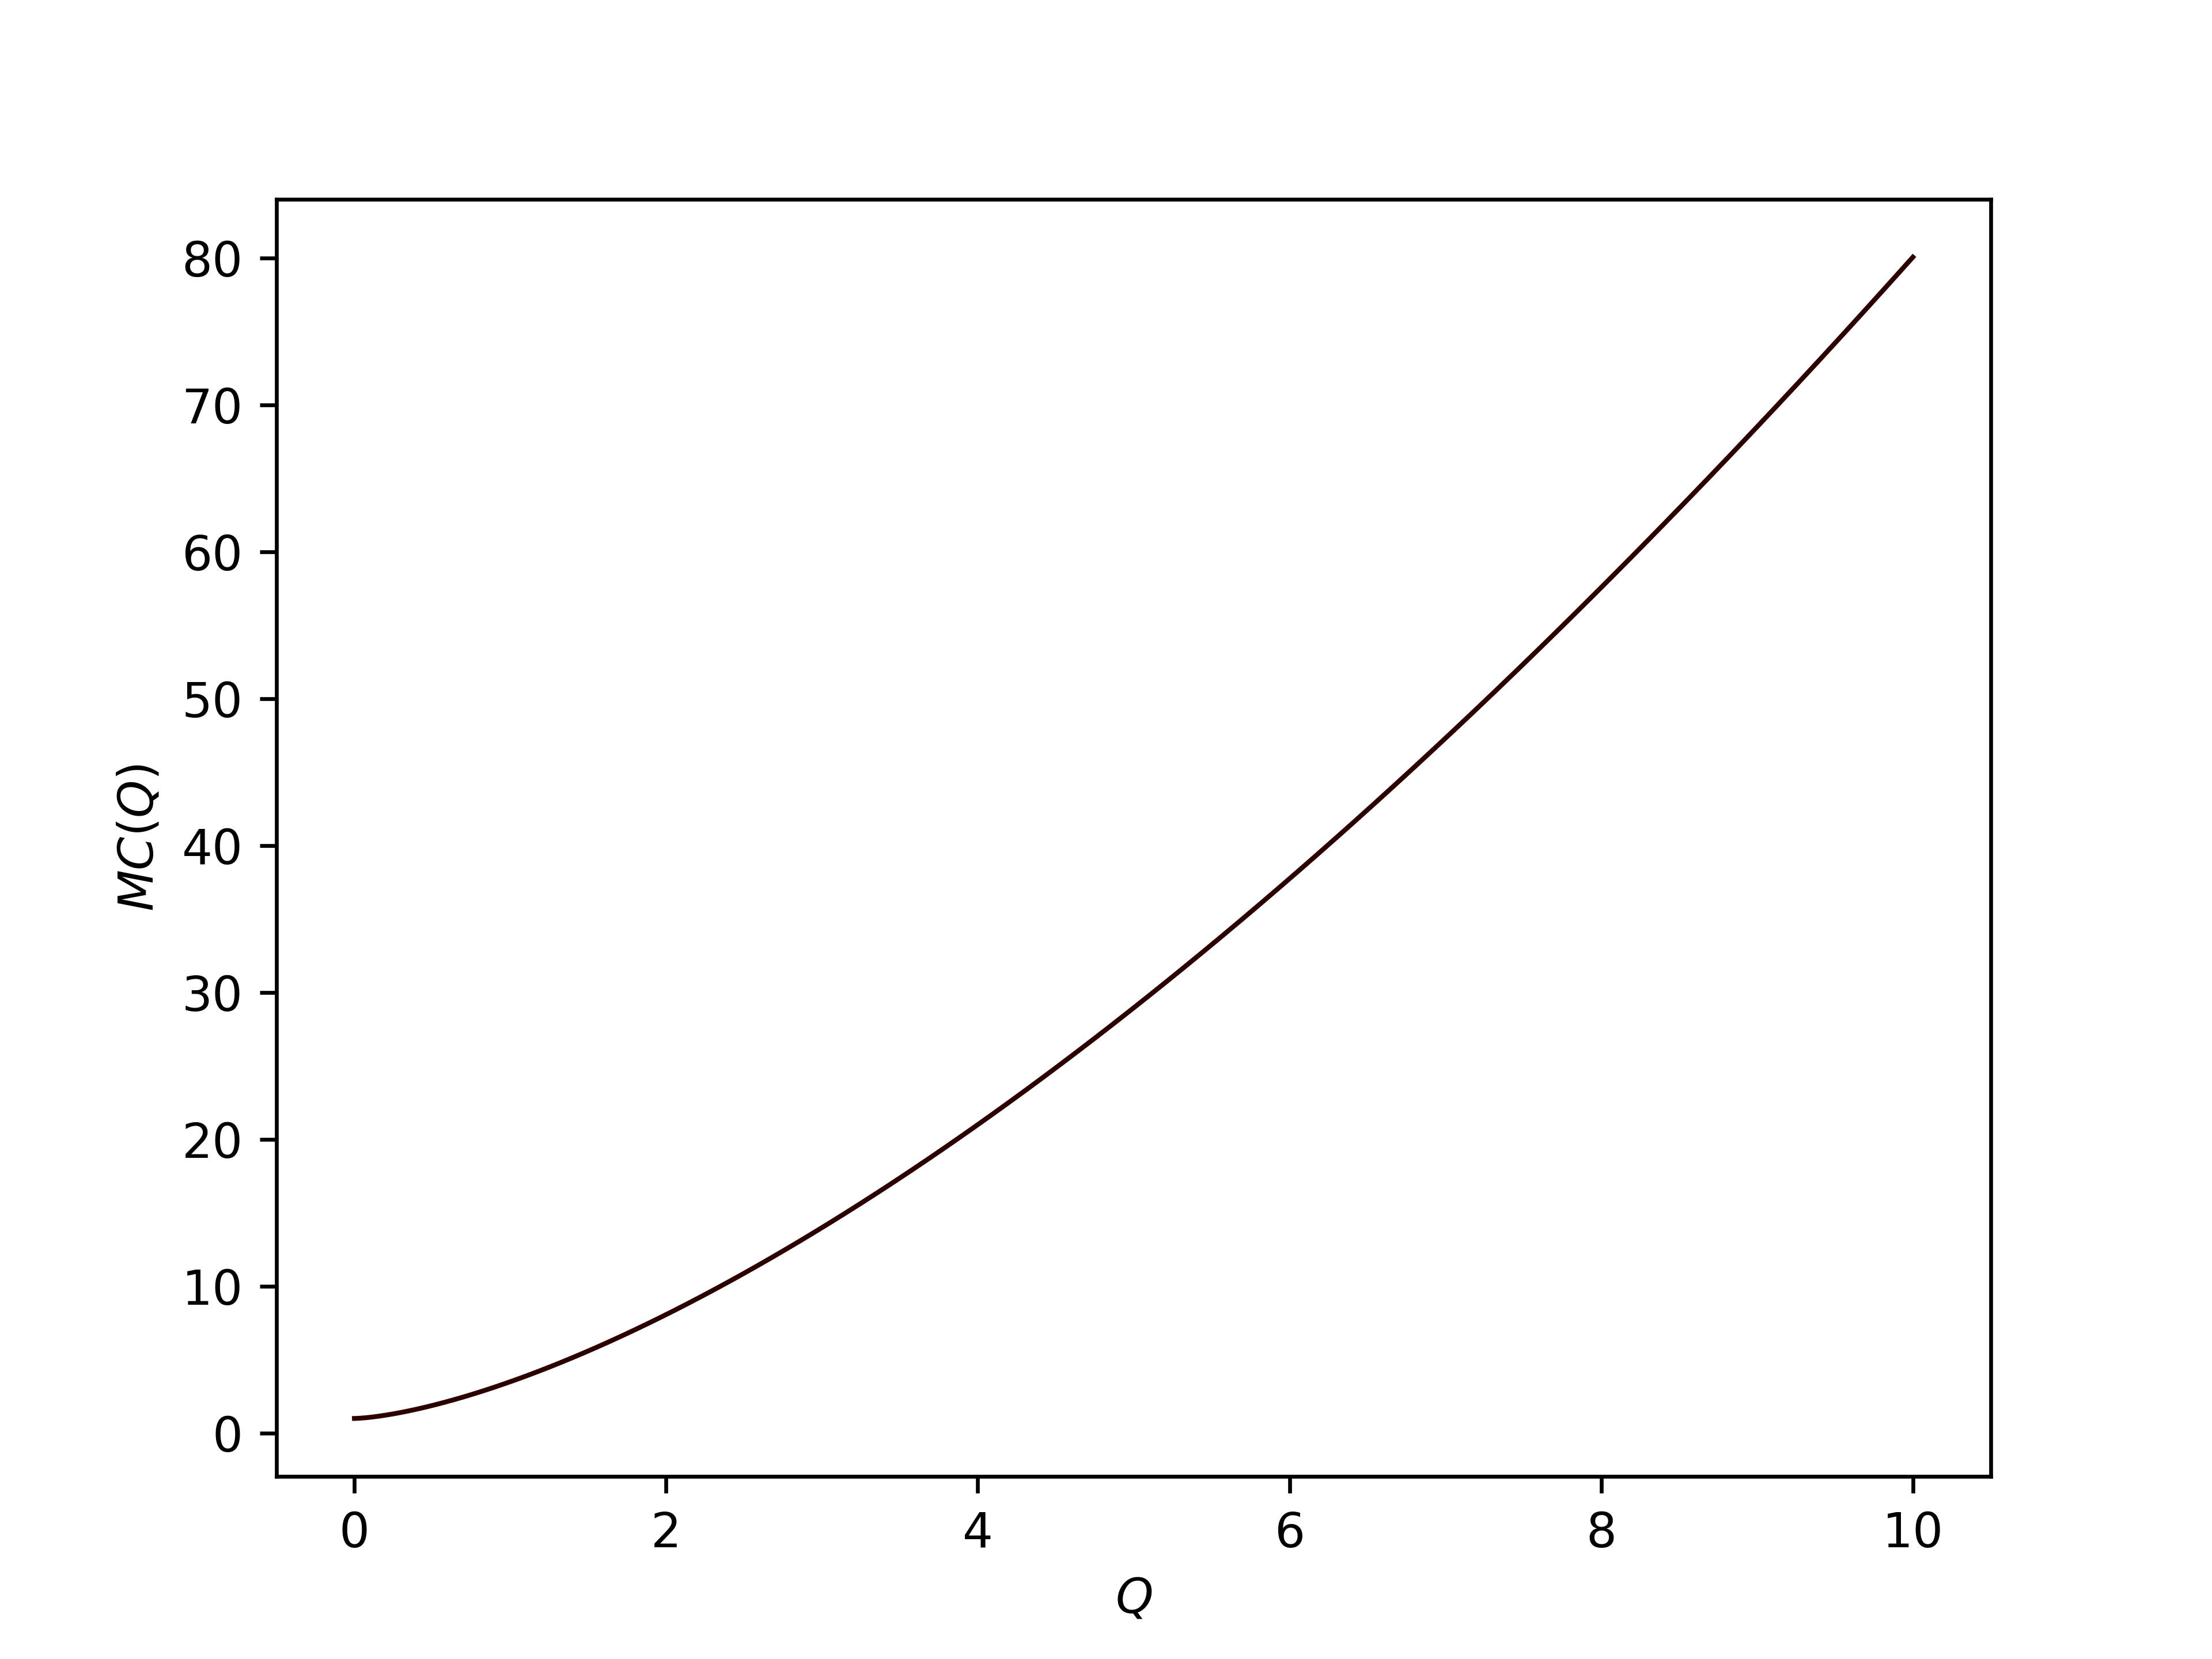
\includegraphics[width=0.8\textwidth]{figures/5_Differentiation/QQ5.png}
\end{figure}

$$
  C''(Q) = a\cdot\frac{15}{4}Q^{\frac{1}{2}} \geq 0 \quad \forall Q \geq 0 \: \therefore \: \text{convex}.
$$

\clearpage

\subsection{Long Questions}

\noindent

1.

a)

$$
  MPL = \frac{\dd y}{\dd n} = 60 - \frac{3}{5}n^2
$$

b)

$$
  y''(n) = -\frac{6}{5}n \leq 0 \quad \forall n \geq 0 \: \therefore \: \text{decreasing returns to labour.}
$$

c)

\begin{center}
  \begin{tabular}{l c c c c}
    $n$ & 1 & 5 & 10 & 15 \\
    $y(n)$ & 59.8 & 275 & 400 & 225 \\
    $A(n) = \frac{y(n)}{n}$ & 59.8 & 55 & 40 & 15 \\
    $MPL(n) = \frac{\dd y(n)}{\dd n}$ & 59.4 & 45 & 0 & -75
  \end{tabular}
\end{center}

d)

"Too many cooks spoil the broth."

e)
















\end{document}
